\documentclass[12pt,a4paper]{article}

% Essential packages
\usepackage[utf8]{inputenc}
\usepackage[T1]{fontenc}
\usepackage[margin=1in]{geometry}
\usepackage{amsmath,amssymb,amsthm}
\usepackage{graphicx}
\usepackage{hyperref}
\usepackage{listings}
\usepackage{xcolor}
\usepackage{enumitem}
\usepackage{fancyhdr}
\usepackage{tcolorbox}
\usepackage{booktabs}
\usepackage{makecell}
\usepackage{placeins}
\usepackage{tabularx}

\usepackage{tikz}
\usetikzlibrary{shapes,arrows,positioning,fit,backgrounds,calc}
\usepackage{rotating}


% Code listing settings
\lstset{
    basicstyle=\ttfamily\small,
    keywordstyle=\color{blue},
    commentstyle=\color{gray},
    stringstyle=\color{red},
    numbers=left,
    numberstyle=\tiny\color{gray},
    stepnumber=1,
    numbersep=5pt,
    backgroundcolor=\color{white},
    showspaces=false,
    showstringspaces=false,
    showtabs=false,
    frame=single,
    tabsize=2,
    captionpos=b,
    breaklines=true,
    breakatwhitespace=false
}

% Custom boxes for teaching
\newtcolorbox{keypoint}{
    colback=blue!5!white,
    colframe=blue!75!black,
    title=Key Point
}

\newtcolorbox{example}{
    colback=green!5!white,
    colframe=green!75!black,
    title=Example
}

\newtcolorbox{exercise}{
    colback=orange!5!white,
    colframe=orange!75!black,
    title=Exercise
}

\newtcolorbox{warning}{
    colback=red!5!white,
    colframe=red!75!black,
    title=Common Pitfall
}

% Theorem environments
\theoremstyle{definition}
\newtheorem{definition}{Definition}[section]
\newtheorem{theorem}{Theorem}[section]
\newtheorem{lemma}[theorem]{Lemma}
\newtheorem{proposition}[theorem]{Proposition}

% Header and footer
\pagestyle{fancy}
\fancyhf{}
\lhead{\coursename}
\rhead{Topic: \topicname}
\cfoot{\thepage}

% Document metadata - CUSTOMIZE THESE
\newcommand{\coursename}{Foundations of Quantitative Social Science Research}
\newcommand{\topicname}{Research Design}
\newcommand{\lecturenum}{Lecture 2-3}
\newcommand{\instructor}{Wanhong Huang}
\newcommand{\semester}{Spring 2025}

\title{\textbf{\coursename} \\ \lecturenum: \topicname}
\author{\instructor}
\date{\semester}

\begin{document}

\maketitle

\tableofcontents
\newpage

%=============================================================================
% SECTION 1: LEARNING OBJECTIVES
%=============================================================================
\section{Learning Objectives}

By the end of this session, students will be able to:

\begin{enumerate}
    \item Understand the foundational logic of quantitative social science research, including the full research lifecycle from question formulation to interpretation and dissemination.
    \item Distinguish major research schemes (e.g., experimental, quasi-experimental, and observational designs) and explain how their structural dimensions constrain measurement, comparison, and inference.
    \item Critically evaluate the identification assumptions underlying different quantitative methods, and assess their plausibility in applied research settings.
    \item Select and justify appropriate measurement strategies and confounding control techniques for their own research questions.
\end{enumerate}

%=============================================================================
% SECTION 2: OVERVIEW
%=============================================================================
\section{Overview}

\begin{keypoint}
Quantitative social science research is not defined by individual methods or tools, but by coherent design choices that link 
research questions, data, methods, and assumptions across the entire research lifecycle.
\end{keypoint}

This session introduces a unified framework for understanding quantitative social science research as an integrated process 
rather than a collection of isolated techniques. We examine how classical research 
designs (such as randomized experiments, cohort studies, and panel designs) and modern 
approaches (including digital trace analysis and adaptive designs) can be systematically compared along shared 
dimensions such as intervention structure, temporal organization, comparison logic, and confounding control.

Rather than focusing on algorithmic details, the emphasis is placed on methodological reasoning: how design choices encode 
assumptions, how measurement modalities shape inference, and how different research schemes achieve (or fail to achieve) 
credible causal and descriptive claims. This perspective provides students with a conceptual map that supports both critical reading of empirical studies and principled design of their own quantitative research projects.





\section{Dimensions for Research Schemes}

Research designs in quantitative social science can be systematically described using a finite set of \emph{design dimensions}. Design dimensions are fundamental, conceptually distinct properties of a study that determine how data are generated, how comparisons are constructed, and what forms of inference are warranted. They are not statistical methods, estimators, or data collection techniques. Instead, dimensions function as \emph{primitive building blocks} from which recognizable research schemes are constructed.

Each empirical study can be represented as a specific configuration of values along these dimensions. While the full Cartesian space of all possible combinations is large, only a subset of combinations is logically coherent, practically feasible, and inferentially meaningful. Stable and recurrent configurations of dimensions give rise to canonical research schemes.

The principal dimensions are described below.

\subsection{Intervention Structure}

The intervention dimension characterizes whether and how the researcher actively manipulates exposure. This is perhaps the most fundamental design dimension, as it determines the degree of researcher control over the treatment assignment process and fundamentally shapes what types of causal inference are possible. In quantitative social science research, the intervention structure delimits the boundary between experimental and non-experimental inquiry, each with distinct epistemic strengths and practical constraints. The intervention dimension strongly constrains the scope of causal inference: experimental designs provide the strongest warrant for causal claims but face ethical and practical limitations, while observational designs offer greater external validity and feasibility at the cost of requiring stronger untestable assumptions.

\subsubsection{Experimental Intervention}

The researcher assigns treatment or exposure directly. Experimental designs afford the strongest claims to internal validity when properly implemented, as the researcher controls the allocation mechanism and can isolate the treatment effect from confounding influences through randomization or other design features. The ability to manipulate treatment allows the researcher to establish clear temporal precedence and to combine assignment with measurement protocols optimized for the research question.

\subsubsection{Quasi-experimental Intervention}

Treatment assignment is externally determined but structured in a way that enables causal comparison. The researcher does not control assignment but exploits systematic variation—such as policy changes, institutional rules, or natural discontinuities—that approximates experimental conditions under specific assumptions. Quasi-experimental designs bridge experimental and observational approaches, leveraging naturally occurring variation while maintaining some structural features that support credible causal inference.

\subsubsection{Observational Design}

No manipulation of exposure occurs. The researcher observes naturally occurring variation in treatment or exposure without intervening in the assignment process. Causal inference in observational settings requires stronger assumptions about the absence of confounding, typically operationalized through statistical adjustment, matching, or other methods that condition on measured covariates. Observational designs are essential when experimental manipulation is infeasible, unethical, or would fundamentally alter the phenomenon of interest.

\subsection{Assignment Mechanism}

The assignment mechanism specifies the process by which units receive treatments or exposures. While closely related to intervention structure, the assignment mechanism is analytically distinct: it describes \emph{how} units come to be exposed, rather than \emph{whether} the researcher controls exposure. This dimension is central to causal inference because the assignment mechanism determines what counterfactual comparisons are credible and what assumptions are required for valid causal identification. Different assignment mechanisms generate different patterns of confounding and selection, which in turn necessitate different identification strategies. Understanding the assignment mechanism is essential for assessing whether treatment and control groups are comparable and for determining what statistical or design-based methods can render them comparable.

\subsubsection{Randomized Assignment}

Allocation is determined by a stochastic process controlled by the researcher. Randomization balances observed and unobserved confounders in expectation, providing the foundation for unconfounded treatment effect estimation. The probability of assignment may be equal across units (simple randomization), vary by strata (stratified randomization), or depend on covariates (covariate-adaptive randomization). Regardless of the specific randomization scheme, the key property is that treatment assignment is statistically independent of potential outcomes.

\subsubsection{Rule-based Assignment}

Allocation follows deterministic rules or thresholds, such that treatment is assigned to all units meeting specified criteria (e.g., all units scoring above a cutoff, all individuals in certain geographic areas, or all applicants meeting eligibility requirements). Rule-based assignment enables identification strategies such as regression discontinuity designs when units near the threshold are comparable. The deterministic nature of assignment means that treatment status is a known function of observed characteristics, which can be exploited for causal inference under appropriate continuity assumptions.

\subsubsection{Natural Assignment}

Allocation is driven by external forces outside researcher control, such as policy implementation, geographic factors, historical events, or institutional processes. Natural assignment may approximate randomization if the assignment mechanism is plausibly exogenous to potential outcomes—that is, if factors determining treatment are unrelated to the outcome except through their effect on treatment receipt. Credibility of causal claims under natural assignment depends critically on substantive arguments about the assignment process and empirical assessment of balance on observed covariates.

\subsubsection{Self-selection}

Units select into exposure based on their own choices, preferences, or characteristics. Self-selection creates endogeneity concerns, as the factors influencing treatment choice (such as motivation, risk preferences, or anticipated benefits) may also directly affect outcomes. This generates confounding that cannot be eliminated by design but must be addressed through modeling assumptions. Controlling for selection-driven confounding requires observing and adjusting for all relevant selection factors, an assumption (conditional independence or selection on observables) that is inherently untestable.

\subsection{Temporal Structure}

Temporal structure captures how observations are distributed over time. This dimension is fundamental to quantitative social science because many theoretical questions concern change, dynamics, and causal processes that unfold temporally. The temporal dimension determines whether a design can establish temporal precedence (a necessary condition for causal inference), track within-unit changes, detect time-varying effects, or distinguish short-term from long-term impacts. Different temporal structures enable different analytical strategies: cross-sectional designs efficiently estimate associations at a point in time; longitudinal designs track change and enable within-unit comparisons; time-series designs capture high-frequency dynamics and enable interrupted time-series analyses. The choice of temporal structure involves tradeoffs among resource requirements, attrition, time-varying confounding, and the ability to address temporally grounded research questions.

\subsubsection{Cross-sectional}

Units are observed at a single point in time. Cross-sectional designs are efficient and avoid attrition but cannot establish temporal precedence between exposure and outcome or distinguish cohort effects from age effects. All variation is between-unit variation, precluding within-unit comparisons.

\subsubsection{Longitudinal}

Units are observed at multiple discrete time points. Longitudinal designs enable analysis of change, assessment of temporal ordering, and estimation of both within-unit and between-unit effects. The interval between observations may range from days to years depending on the process under study.

\subsubsection{Time-series}

Units are observed at high-frequency or continuously over time. Time-series designs capture fine-grained temporal dynamics, enable detection of short-term fluctuations and long-term trends, and support methods such as interrupted time-series analysis that exploit detailed pre-intervention baselines.

\subsection{Unit Tracking}

Unit tracking describes whether the same observational units are followed over time. This dimension is distinct from temporal structure: a study may be longitudinal (multiple time points) but use repeated cross-sections (different units each time) or follow the same panel of units. Unit tracking determines what sources of variation are available for analysis and what types of unobserved heterogeneity can be controlled. Panel designs, which follow the same units, enable differencing out time-invariant unobserved confounders through fixed effects methods, but face challenges from attrition and the need to model time-varying confounding. Repeated cross-sections avoid attrition but cannot exploit within-unit variation. Cohort designs balance some advantages of both by following a defined group without requiring full panel structure. This dimension critically affects identification strategies and the types of causal questions that can be addressed.

\subsubsection{Repeated Cross-sections}

Different units are observed at each time point. Repeated cross-sectional designs can track aggregate-level changes and cohort dynamics without the cost and attrition challenges of panel data, but cannot identify within-unit changes or control for unit-specific unobserved heterogeneity.

\subsubsection{Panel Designs}

The same units are repeatedly observed across all measurement occasions. Panel designs enable within-unit comparisons that control for stable unobserved characteristics, but require strategies to address selective attrition and time-varying confounding.

\subsubsection{Cohort Designs}

Units defined by a shared entry condition (e.g., birth year, program entry date, exposure to a common event) are followed over time. Cohort designs may involve complete panel tracking or accept some attrition, and naturally control for cohort-level confounders while allowing analysis of within-cohort heterogeneity.

\subsection{Directionality of Inquiry}

Directionality refers to the temporal relationship between exposure measurement and outcome observation. This dimension is crucial for quantitative social science because it determines vulnerability to specific types of bias—particularly recall bias, social desirability bias, and reverse causation—and affects the credibility of causal inference. Prospective designs measure exposure before outcome occurrence, establishing clear temporal precedence and minimizing recall distortion. Retrospective designs work backward from observed outcomes to assess prior exposures, which is efficient for rare outcomes but vulnerable to differential recall and selection bias. Simultaneous measurement precludes establishing temporal ordering altogether, limiting causal interpretation unless strong assumptions or external information justify claims about directionality. The choice of directionality involves tradeoffs between bias, cost, and feasibility.

\subsubsection{Prospective}

Exposure precedes outcome observation in both the causal process and the data collection sequence. Prospective designs establish clear temporal precedence, minimize recall bias in exposure measurement, and enable real-time data collection. However, they may require long follow-up periods and are inefficient for studying rare outcomes.

\subsubsection{Retrospective}

Outcome status determines exposure assessment: researchers identify individuals with the outcome of interest and then ascertain their prior exposure history. Retrospective designs are efficient for rare outcomes and can be implemented quickly, but are susceptible to recall bias (differential memory of exposure by outcome status), selection bias (if outcome occurrence affects study inclusion), and survivor bias (if individuals must survive to outcome occurrence to be included).

\subsubsection{Simultaneous}

Exposure and outcome are measured concurrently, typically in cross-sectional surveys or assessments. Simultaneous measurement cannot establish temporal precedence from the design itself, making causal inference reliant on strong assumptions about the direction of causality, auxiliary information from theory or external studies, or structural modeling assumptions.

\subsection{Comparison Logic}

The comparison logic defines the source of the counterfactual—that is, how the design constructs an answer to the question "compared to what?" In causal inference, we seek to compare observed outcomes under treatment to counterfactual outcomes under control. Since the counterfactual is never directly observed, research designs use various comparison strategies to approximate it. The comparison logic determines what types of confounding the design can address and what assumptions are required. Between-unit comparisons assume different units are comparable (exchangeability); within-unit comparisons assume units are comparable to themselves at different times (temporal stability); historical comparisons assume the past predicts the counterfactual future (trend continuity); external comparisons assume other contexts are informative (transferability). Different comparison logics support different identification strategies and have characteristic vulnerabilities.

\subsubsection{Between-unit Comparisons}

Different units serve as comparisons for one another. Between-unit designs compare treated and untreated individuals, groups, or other entities. Validity requires that units are exchangeable—that is, comparable in terms of potential outcomes. This may be achieved through randomization, matching, statistical adjustment, or design-based strategies that render units comparable.

\subsubsection{Within-unit Comparisons}

Units serve as their own controls, comparing outcomes for the same unit at different times or under different conditions. Within-unit comparisons control for all time-invariant characteristics of the unit, observed and unobserved, but require assumptions about temporal stability and are vulnerable to time-varying confounding, carryover effects, and secular trends.

\subsubsection{Historical Comparisons}

Past observations act as counterfactuals for present or future outcomes. Historical comparisons, common in interrupted time-series and difference-in-differences designs, assume that pre-intervention trends would have continued absent intervention. Validity requires correct extrapolation of historical patterns into the counterfactual future.

\subsubsection{External Comparisons}

Other populations, contexts, or settings provide benchmarks for comparison (e.g., comparing one country to another, or study population outcomes to national norms). External comparisons rely on assumptions about the transferability of causal effects or the comparability of populations across contexts, assumptions that are often difficult to justify without strong theory or auxiliary evidence.

\subsection{Data Provenance}

Data provenance specifies the origin of the data used in analysis. This dimension affects data quality, construct validity, measurement error, completeness, and the alignment between measurement and theoretical constructs. Primary data are collected specifically for the research question at hand, allowing researchers to optimize measurement instruments, sampling, and timing for their inferential goals, but at substantial cost. Secondary data were generated for other purposes—administrative operations, prior research, commercial transactions—and may be available at low cost and large scale, but often involve compromises in construct validity and completeness. Understanding data provenance is essential for assessing measurement validity, anticipating missing data patterns, and evaluating whether available variables adequately operationalize theoretical constructs.

\subsubsection{Primary Data}

Collected specifically for the study. Primary data collection allows researchers to tailor instruments to theoretical constructs, optimize measurement timing, and implement quality control procedures. However, primary data collection is resource-intensive and may face challenges of recruitment, response rates, and attrition in longitudinal designs.

\subsubsection{Secondary Data}

Originally collected for other purposes, such as administrative operations, prior research studies, or commercial activities. Secondary data offer cost efficiency and often provide access to large samples or populations, but may involve construct validity concerns (available measures may not align well with theoretical constructs), missing data on key variables, and limited control over data quality.

\subsubsection{Mixed Sources}

Combination of primary and secondary data, such as linking survey responses to administrative records, augmenting administrative data with targeted primary data collection, or merging multiple secondary data sources. Mixed-source designs can capitalize on the strengths of each data type while potentially addressing their respective limitations, though linkage itself introduces challenges of matching accuracy and consent.

\subsection{Sampling Strategy}

Sampling strategy determines how units are selected from the target population into the study sample. This dimension governs external validity (the ability to generalize findings beyond the study sample) and the justification for statistical inference to broader populations. Probability sampling provides a foundation for design-based inference and enables quantification of sampling uncertainty, but may be costly or infeasible for many populations. Non-probability sampling is more flexible and accessible but limits formal generalization to target populations. The sampling dimension interacts with other design features: population-representative samples enhance external validity but may complicate causal inference if they include substantial heterogeneity; convenience samples may enable cleaner causal estimates in homogeneous subgroups but raise questions about generalizability. Understanding sampling strategy is essential for interpreting study findings and assessing the populations to which results apply.

\subsubsection{Probability Sampling}

Units are selected with known, non-zero probability. Probability sampling methods include simple random sampling, stratified sampling (random sampling within strata defined by covariates), cluster sampling (random sampling of groups followed by observation of all or a sample of units within clusters), and multistage designs. Probability sampling supports design-based inference, allows calculation of sampling weights to adjust for unequal selection probabilities, and provides a basis for standard error estimation that accounts for the sampling design.

\subsubsection{Non-probability Sampling}

Units are selected without a probabilistic basis. Non-probability methods include convenience sampling (units that are readily accessible), purposive sampling (deliberate selection of information-rich cases), quota sampling (non-random selection to fill predetermined quotas), and snowball sampling (chain-referral sampling). Non-probability samples may be suitable for exploratory research, hypothesis generation, or studies focusing on specific subpopulations, but do not support formal statistical inference to a defined population without strong assumptions.

\subsubsection{Census}

All units in the target population are included. Census designs eliminate sampling error and maximize statistical power, but are often feasible only for small, well-defined populations (e.g., all students in a school, all firms in an industry sector). Census data may still face coverage error if population enumeration is incomplete.

\subsubsection{Selective Enrollment}

Units meeting specific eligibility criteria are enrolled, often combining elements of purposive selection with probability or convenience sampling among eligible units. Selective enrollment is common in clinical trials (eligibility criteria ensure safety and relevance), evaluation studies (target program-eligible populations), and studies requiring specific characteristics for theoretical reasons. Selective enrollment affects generalizability to broader populations.

\subsection{Unit of Analysis and Observation}

This dimension distinguishes between the level at which data are collected (unit of observation) and the level at which inferences are made (unit of analysis). Misalignment between these levels creates aggregation or disaggregation challenges and potential logical fallacies. This dimension is particularly important in quantitative social science because social phenomena are inherently multilevel: individuals nested in families, students in classrooms, workers in firms, citizens in nations. The choice of analytical level affects what questions can be addressed, what confounders must be considered, and what statistical methods are appropriate. Aggregate analyses may obscure individual-level heterogeneity; individual analyses may fail to capture contextual or compositional effects. Ecological fallacy (inferring individual-level relationships from aggregate data) and atomistic fallacy (ignoring higher-level structure) are key threats when observation and analysis units are misaligned.

\subsubsection{Individual-level}

Individuals serve as both observation and analysis units. Individual-level designs directly model individual outcomes and characteristics, providing maximum resolution for heterogeneity in treatment effects and outcomes. Standard regression methods and most causal inference techniques are designed for individual-level data.

\subsubsection{Aggregate-level}

Groups, organizations, or geographic units (e.g., schools, firms, neighborhoods, countries) are the units of both observation and analysis. Aggregate-level designs are appropriate when the theoretical question concerns collective entities or when individual data are unavailable. Aggregate analysis may be necessary for policy-relevant questions about organizational or jurisdictional effects.

\subsubsection{Multilevel}

Observations are nested within higher-level units, requiring hierarchical or multilevel modeling that explicitly represents this structure. Multilevel designs allow decomposition of variance across levels, estimation of cross-level interactions, and appropriate quantification of uncertainty that accounts for clustering. Multilevel analysis addresses questions about contextual effects and compositional effects while avoiding aggregation bias.

\subsubsection{Ecological}

Aggregate data are used to make inferences about aggregate-level processes or relationships. Ecological designs analyze associations among variables measured at the group level (e.g., relationships between county-level characteristics and county-level outcomes). Ecological inference is valid for understanding aggregate patterns but requires strong assumptions if used to infer individual-level relationships.

\subsection{Measurement Modality}

The measurement modality dimension characterizes how key variables are observed and recorded. This dimension has profound implications for measurement validity (whether measures capture intended constructs), reliability (consistency of measurement), and bias (systematic error in measurement). Different modalities involve distinct tradeoffs among objectivity, construct validity, cost, participant burden, and ethical considerations. In quantitative social science, where many constructs of interest (attitudes, behaviors, social processes) are not directly observable, measurement modality choices fundamentally shape what can be studied and how credibly. The measurement dimension interacts with other design features: experimental designs often justify costly objective measures; observational studies often rely on self-report or administrative data; longitudinal designs must balance measurement burden against attrition. Understanding measurement error structure by modality is essential for assessing threats to validity and for selecting appropriate statistical methods.

\subsubsection{Direct Observation}

Researchers or trained observers record behaviors, events, or conditions in real time through systematic observation protocols. Examples include classroom observation schedules, workplace time-motion studies, structured field observations, and behavioral coding in laboratory settings. Direct observation minimizes recall bias and provides objective behavioral measurement, but is labor-intensive, may involve observer effects (reactivity), requires high inter-rater reliability, and is limited to observable behaviors rather than internal states or subjective experiences.

\subsubsection{Self-report}

Respondents provide information about themselves through surveys, interviews, or questionnaires. This includes standardized instruments (validated scales), open-ended interviews, ecological momentary assessment (repeated sampling of current states), and retrospective reports of past events or behaviors. Self-report provides access to internal experiences, subjective states, and private behaviors not accessible through observation, but is subject to recall bias, social desirability bias, acquiescence bias, satisficing, and question wording effects. The structure and quality of self-report measures vary widely, from rigorously validated psychometric instruments to ad hoc single-item questions.

\subsubsection{Proxy Report}

Information is obtained from knowledgeable informants rather than directly from the target individual. Examples include teachers reporting on student behavior, parents reporting on children's development, or family members reporting on patients' health status. Proxy reports may provide information when self-report is not feasible (young children, cognitively impaired individuals) or may triangulate with self-report to improve measurement. However, proxy reports may diverge from self-reports due to limited observability of internal states or private behaviors, differential interpretation of questions, or differing perspectives and incentives.

\subsubsection{Administrative Records}

Data are extracted from institutional or governmental databases created for operational purposes. Examples include health records (diagnoses, procedures, prescriptions), educational transcripts (grades, test scores, attendance), tax records (income, employment), criminal justice data (arrests, convictions, incarceration), and vital statistics (births, deaths, marriages). Administrative data offer objectivity, large scale, population coverage, and longitudinal tracking, but may suffer from recording errors, systematic missingness related to system contact, construct validity challenges when operational categories do not align with research constructs, and changes in recording practices over time.

\subsubsection{Biomarkers and Physiological Measures}

Biological specimens or physiological sensors provide objective measures of physical states or biological processes. Examples include cortisol levels (stress), blood pressure, neuroimaging (brain structure and function), genetic markers, and cardiovascular or metabolic indicators. Biomarkers reduce self-report bias, provide objective indicators of physiological processes, and may capture information not accessible through self-report. However, they require specialized equipment and expertise, involve participant burden and potential health risks, may raise privacy concerns (especially genetic data), and often serve as imperfect proxies for constructs of theoretical interest (e.g., cortisol as a measure of stress).

\subsubsection{Digital Trace Data}

Passively collected behavioral data from digital platforms, sensors, or transaction systems. Examples include social media activity (posts, likes, network connections), GPS trajectories (mobility patterns), online purchases (consumer behavior), web browsing (information seeking), sensor networks (environmental exposures), and smartphone data (app usage, communication patterns). Digital traces offer high temporal resolution, ecological validity (naturalistic behavior), massive scale, and reduced participant burden (passive collection). However, they raise construct validity concerns (do observed behaviors map onto theoretical constructs?), privacy and ethical issues, selection bias (participation in platforms), algorithmic confounding (platform algorithms affect observed behavior), and heterogeneity in measurement across user populations.

\subsubsection{Performance Tests}

Standardized assessments or experimental tasks measure latent constructs through behavioral performance. Examples include cognitive ability tests (IQ, working memory), achievement tests (math, reading), physical fitness assessments, experimental economic games (risk preferences, cooperation), and implicit association tests (implicit attitudes). Performance tests provide objective behavioral measures of constructs that cannot be directly observed, often with established psychometric properties. However, they may be sensitive to testing conditions, require careful validation, and may not generalize beyond the testing context.

\subsubsection{Mixed Measurement}

Multiple measurement modalities are combined to triangulate constructs or validate measures. Examples include self-reported health combined with biomarkers and medical records, survey responses linked to administrative employment data, or direct observation combined with self-report interviews. Mixed measurement can capitalize on the strengths of different modalities, provide convergent validation, and enable assessment of measurement error through comparison across methods. However, mixed-mode designs introduce complexities of data linkage, require managing discrepancies across measures, and may face challenges of consent for linking data sources.

The choice of measurement modality involves tradeoffs among validity, reliability, cost, participant burden, and ethical considerations. Objective measures (biomarkers, administrative records) reduce certain biases but may not capture subjective states or meanings. Self-report provides access to internal experiences but introduces response biases. Digital traces offer scale and naturalism but complicate construct interpretation. Measurement error structure varies systematically by modality: self-report tends toward systematic bias, administrative records toward random missingness, and digital traces toward measurement heterogeneity across subgroups.

\subsection{Confounding Control Strategy}

The confounding control dimension specifies how the design addresses potential confounding—the presence of common causes of treatment and outcome that threaten causal identification. Confounding is perhaps the central challenge in causal inference: if treatment and outcome share common causes, observed associations may reflect these shared causes rather than causal effects of treatment. The control strategy determines what assumptions must hold for valid causal inference and fundamentally shapes the credibility of causal claims. This dimension is crucial in quantitative social science because most social phenomena involve complex causal networks with multiple pathways connecting exposures to outcomes. Different control strategies embed identifying assumptions in different ways: randomization eliminates confounding by design; design-based identification exploits structural features to approximate randomization; statistical adjustment relies on conditioning on measured confounders. Understanding the confounding control dimension is essential for evaluating whether a study's causal claims are justified and for determining what sensitivity analyses or robustness checks are needed.

\subsubsection{Randomization-based Control}

Random assignment of treatment eliminates confounding by ensuring treatment is statistically independent of all potential confounders, observed and unobserved. Randomization balances confounders in expectation, making treatment and control groups exchangeable and allowing causal effects to be estimated by simple mean differences (or regression adjustment to improve precision). This is the gold standard for internal validity because it requires no assumptions about which variables confound the relationship or how they operate. However, randomization is not always feasible (cannot randomize structural characteristics like race or gender), ethical (cannot randomize harmful exposures), or practical (cannot randomize many policy interventions). Even when feasible, randomization addresses only confounding, not other threats to validity such as attrition, measurement error, or spillover effects.

\subsubsection{Design-based Identification}

The research design exploits structural features that approximate randomization or render confounding implausible under explicit assumptions. Design-based approaches embed identifying assumptions in the design rather than in the statistical model, often providing more credible causal inference than pure statistical adjustment. Each design-based method relies on specific identifying assumptions:

\paragraph{Regression Discontinuity.} Units just above and below a threshold are assumed comparable, isolating treatment effects at the cutoff. Identification requires continuity of potential outcomes at the threshold: individuals on either side differ only in treatment status, not in other characteristics affecting outcomes. RDD provides credible local causal effects but limited generalizability beyond the threshold region.

\paragraph{Instrumental Variables.} An instrument affects the outcome only through its effect on treatment, breaking the confounding pathway. Identification requires instrument relevance (strong first stage), exclusion restriction (instrument affects outcome only through treatment), and independence (instrument uncorrelated with potential outcomes). IV estimates local average treatment effects for compliers—units whose treatment status is affected by the instrument.

\paragraph{Difference-in-Differences.} Treatment and control groups share parallel counterfactual trends, allowing differencing to remove time-invariant confounding. Identification requires that treated and control groups would have followed parallel trends absent treatment. DiD controls for time-invariant confounding and common shocks but is vulnerable to time-varying confounding and violations of parallel trends.

\paragraph{Interrupted Time Series.} Pre-intervention trends establish the counterfactual trajectory absent intervention. Identification requires that the pre-intervention trend would have continued absent intervention and that no concurrent events affect outcomes. ITS provides strong internal validity when long pre-intervention baselines establish stable trends, but is vulnerable to concurrent events and structural changes.

\paragraph{Natural Experiments.} Exogenous shocks or policy changes create as-if random variation in exposure. Identification requires that the natural assignment mechanism is plausibly exogenous—that is, uncorrelated with potential outcomes except through treatment. Credibility depends on substantive arguments about the assignment process and empirical assessment of balance.

Each design-based approach relies on specific identifying assumptions that must be empirically assessed (through balance tests, placebo tests, or sensitivity analyses) and theoretically justified.

\subsubsection{Restriction and Stratification}

Analysis is restricted to units with similar values of known confounders, or conducted separately within strata defined by confounders. Restriction eliminates confounding by the restricted variables through design: if analysis includes only units of a given age, then age cannot confound the relationship. Similarly, stratified analysis ensures comparisons are made only within homogeneous strata. Restriction controls for observed confounders without requiring functional form assumptions, but does not address unmeasured confounders, reduces sample size and generalizability, and may introduce selection bias if restriction is based on post-treatment variables.

\subsubsection{Matching}

Treated and control units are paired or weighted to achieve balance on observed covariates. Matching methods include exact matching (pairing on identical covariate values), propensity score matching (pairing on predicted probability of treatment), coarsened exact matching (matching on coarsened covariates), and genetic matching (optimizing balance metrics). Matching controls for observed confounders by constructing a comparison group that resembles the treated group on measured characteristics. However, matching assumes no unobserved confounding (conditional independence given matched variables) and requires sufficient overlap (common support): for every treated unit there must exist comparable control units. Matching is often combined with regression adjustment (doubly robust estimation) to improve robustness.

\subsubsection{Statistical Adjustment}

Confounders are controlled through regression modeling, inverse probability weighting, or doubly robust estimation. Statistical adjustment conditions on observed confounders, estimating treatment effects within levels of confounders and then aggregating across levels. The validity of statistical adjustment depends on three assumptions: (1) conditional independence—all confounders are observed and included in the model; (2) correct functional form—the relationship between confounders, treatment, and outcome is correctly specified; and (3) positivity—all covariate combinations have non-zero probability of receiving each treatment level. Statistical adjustment is flexible and can accommodate continuous confounders and complex covariate patterns, but relies on strong untestable assumptions (especially conditional independence) and may be sensitive to model misspecification.

\subsubsection{Fixed Effects}

Within-unit or within-cluster variation is exploited to difference out time-invariant or unit-invariant confounders. Fixed effects models include unit-specific intercepts that absorb all stable characteristics of the unit, observed and unobserved. By comparing units to themselves over time (or clusters to themselves across observations), fixed effects control for all time-invariant confounding. Fixed effects are particularly powerful when important confounders are stable characteristics (ability, personality, neighborhood factors). However, fixed effects cannot identify effects of time-invariant treatments, are vulnerable to time-varying confounding, may exacerbate measurement error, and require correct specification of time-varying dynamics.

\subsubsection{Sensitivity Analysis}

Rather than eliminating confounding, sensitivity analyses quantify how strong unmeasured confounding would need to be to overturn the observed association. Sensitivity analysis methods include bounding approaches (calculating bounds on treatment effects under assumed confounding), tipping point analyses (determining the confounding strength required to nullify results), instrumental variable-based sensitivity tests, and simulated confounding scenarios. Sensitivity analysis does not resolve confounding but provides transparency about the robustness of causal claims to violations of identifying assumptions. Strong sensitivity analysis results (effects robust to substantial confounding) strengthen causal inference; weak results (effects eliminated by modest confounding) highlight the fragility of causal claims.

\subsubsection{Negative Controls}

Negative control outcomes (outcomes that should not be affected by treatment) or negative control exposures (exposures that should not affect the outcome) are used to detect residual confounding. If negative controls show associations with treatment or outcome, this suggests that confounding is present: the associations cannot be causal (by definition of negative controls) and therefore must reflect confounding or bias. Negative controls provide empirical evidence about the adequacy of confounding control without requiring explicit identification of confounders. However, specifying valid negative controls requires strong substantive assumptions about what should and should not be causally related.

\subsubsection{No Explicit Control}

Some observational studies make no systematic attempt to control confounding, either because the research question is purely descriptive (not causal) or because causal interpretation relies on conditional independence assumptions implicit in the research question. Studies without explicit confounding control may still provide valuable descriptive evidence, generate hypotheses, or inform causal inference when combined with theory or evidence from other sources. However, causal claims from such studies are generally weak and require strong justification.

The choice of confounding control strategy is central to causal inference. Randomization-based and design-based strategies embed identifying assumptions in the research design itself, while statistical adjustment and matching embed assumptions in the analysis model. Transparent articulation of the chosen strategy and its underlying assumptions is essential for evaluating the credibility of causal claims. Multiple strategies may be combined in a single study. For example, a difference-in-differences design may additionally employ matching to improve covariate balance or regression adjustment to control for time-varying confounders. Combining strategies can provide robustness checks and strengthen causal inference if results are consistent across methods with different assumptions.


Multiple strategies may be combined in a single study. For example, a difference-in-differences design may additionally employ matching to improve covariate balance or regression adjustment to control for time-varying confounders.

\subsection{Summary Table: Research Design Dimensions}

\begin{table}[!t]
\centering
\caption{Taxonomy of Research Design Dimensions}
\label{tab:dimensions}
\small
\renewcommand{\arraystretch}{1.15}
\begin{tabular}{p{7cm}p{7cm}}
\hline
\textbf{Dimension} & \textbf{Possible Values} \\
\hline
Intervention Structure &
\makecell[l]{Experimental \\ Quasi-experimental \\ Observational} \\ \hline

Assignment Mechanism &
\makecell[l]{Randomized \\ Rule-based \\ Natural \\ Self-selection} \\ \hline

Temporal Structure &
\makecell[l]{Cross-sectional \\ Longitudinal \\ Time-series} \\ \hline

Unit Tracking &
\makecell[l]{Repeated cross-sections \\ Panel \\ Cohort} \\ \hline

Directionality of Inquiry &
\makecell[l]{Prospective \\ Retrospective \\ Simultaneous} \\ \hline
\end{tabular}
\end{table}


\begin{table}[!t]
\centering
\caption{Taxonomy of Research Design Dimensions (Continued)}
\small
\renewcommand{\arraystretch}{1.15}
\begin{tabular}{p{7cm}p{7cm}}
\hline
\textbf{Dimension} & \textbf{Possible Values} \\
\hline
Comparison Logic &
\makecell[l]{Between-unit \\ Within-unit \\ Historical \\ External} \\ \hline

Data Provenance &
\makecell[l]{Primary \\ Secondary \\ Mixed sources} \\ \hline

Sampling Strategy &
\makecell[l]{Probability \\ Non-probability \\ Census \\ Selective enrollment} \\ \hline

Unit of Analysis &
\makecell[l]{Individual-level \\ Aggregate-level \\ Multilevel \\ Ecological} \\ \hline

Measurement Modality &
\makecell[l]{Direct observation \\ Self-report \\ Proxy report \\ Administrative records \\ Biomarkers \\ Digital trace data \\ Performance tests \\ Mixed measurement} \\ \hline

Confounding Control &
\makecell[l]{Randomization-based \\ Design-based identification \\ Restriction / stratification \\ Matching \\ Statistical adjustment \\ Fixed effects \\ Sensitivity analysis \\ Negative controls \\ No explicit control} \\ \hline
\end{tabular}
\end{table}



\subsection{Interdependencies Among Dimensions}

Design dimensions are not fully independent. Certain dimensional values constrain or necessitate others, creating structural dependencies that shape the feasible design space.

\textbf{Logical dependencies}: Some combinations are logically impossible. Randomized assignment requires experimental or quasi-experimental intervention structure; retrospective directionality is incompatible with randomization; within-unit comparisons require longitudinal temporal structure.

\textbf{Practical dependencies}: Certain combinations, while not logically impossible, are rarely implemented due to practical constraints. For example, randomized experiments typically use primary data collection; meta-analyses necessarily use secondary data; digital trace studies typically employ observational designs.

\textbf{Inferential dependencies}: The choice along one dimension affects which values are appropriate on other dimensions for valid inference. High-frequency time-series data may enable design-based identification strategies (e.g., interrupted time series) that are infeasible with cross-sectional data. Panel data enable fixed effects control that cross-sectional designs cannot support.

\textbf{Measurement-design dependencies}: Certain measurement modalities align naturally with particular design structures. Biomarkers and performance tests are common in experimental designs where precise measurement justifies the cost. Digital trace data typically appear in observational designs with natural assignment. Administrative records often enable large-scale quasi-experimental designs exploiting policy variation.

\textbf{Control strategy dependencies}: The feasibility and appropriateness of confounding control strategies depend on other dimensional values. Randomization-based control defines experimental intervention structure. Design-based identification requires specific temporal structures (longitudinal for DiD, cross-sectional with threshold for RDD). Fixed effects require panel data. Matching and statistical adjustment require rich covariate measurement.

Understanding these interdependencies helps researchers navigate the design space efficiently and avoid internally inconsistent configurations.



\section{Research Schemes Taxonomy}

Research schemes are coherent, recognizable configurations of design dimensions that support specific inferential goals. Unlike dimensions, which are abstract descriptors, research schemes function as \emph{inferential templates}. Each scheme is associated with characteristic assumptions, strengths, and limitations.

This section presents a taxonomy of commonly used research schemes in quantitative social science.

\subsection{Randomized Controlled Trials}

Randomized controlled trials combine experimental intervention with randomized assignment and prospective outcome measurement. Comparisons are typically between treatment and control groups, though within-unit designs (e.g., crossover trials) may also be employed.

RCTs provide strong internal validity under correct implementation, but may face constraints related to ethics, feasibility, and external validity. Common variants include parallel group designs, cluster-randomized trials, factorial designs, and adaptive randomization schemes.

\textbf{Dimensional configuration}: Experimental intervention, randomized assignment, prospective directionality, between-unit (or within-unit) comparison, primary data collection, randomization-based confounding control, typically direct observation or performance tests for outcomes.

\textbf{Key identifying assumption}: Random assignment ensures treatment independence from potential outcomes (unconfoundedness by design).

\subsection{Quasi-Experimental Designs}

Quasi-experimental designs exploit structured variation in exposure without full randomization. Common examples include difference-in-differences, regression discontinuity designs, instrumental variables, and interrupted time-series analyses.

These designs rely on design-specific assumptions, such as parallel trends or continuity at thresholds, to support causal inference. Each variant has characteristic data requirements and identifying assumptions.

\textbf{Dimensional configuration}: Quasi-experimental intervention, rule-based or natural assignment, longitudinal or cross-sectional temporal structure, between-unit and/or within-unit comparison, primary or secondary data, design-based identification for confounding control.

\textbf{Key identifying assumptions}: Vary by specific design (e.g., parallel trends for DiD, continuity at threshold for RDD, exclusion restriction for IV).

\subsection{Cohort Studies}

Cohort studies follow a group of units defined by a shared initial condition over time, typically in an observational setting. Exposure is measured prior to outcome observation, enabling prospective analysis of risk and incidence.

While cohort designs support temporal ordering, they remain vulnerable to confounding. Cohort studies may employ restriction, statistical adjustment, or matching to control confounding.

\textbf{Dimensional configuration}: Observational, natural or self-selection assignment, longitudinal temporal structure, cohort tracking, prospective directionality, between-unit comparison, primary data, statistical adjustment or restriction for confounding control, typically self-report or biomarkers for exposure and outcomes.

\textbf{Key identifying assumption}: Conditional independence given measured covariates (no unmeasured confounding).

\subsection{Case--Control Studies}

Case--control studies select units based on outcome status and retrospectively assess exposure. Comparisons are made between cases and controls to identify associations with the outcome of interest.

These designs are efficient for rare outcomes but are susceptible to selection and recall bias. Case-control studies typically use matching on key confounders and statistical adjustment in analysis.

\textbf{Dimensional configuration}: Observational, selective enrollment based on outcome status, cross-sectional or retrospective temporal structure, retrospective directionality, between-unit comparison, primary or secondary data, matching and statistical adjustment for confounding control, often self-report or administrative records for exposure.

\textbf{Key identifying assumptions}: Controls represent the source population that gave rise to cases; exposure measurement is unbiased by outcome status; conditional independence given covariates.

\subsection{Cross-Sectional Studies}

Cross-sectional studies observe units at a single point in time, measuring exposures and outcomes simultaneously. They are primarily descriptive and correlational in nature.

Causal interpretation is generally limited without additional assumptions or external information. When causal claims are made, they typically rely on statistical adjustment or instrumental variables.

\textbf{Dimensional configuration}: Observational, self-selection or natural assignment, cross-sectional temporal structure, simultaneous directionality, between-unit comparison, primary or secondary data, statistical adjustment if causal inference attempted, self-report or administrative records common.

\textbf{Key limitation}: Cannot establish temporal precedence; vulnerable to reverse causation.

\subsection{Panel Studies}

Panel studies repeatedly observe the same units over time without experimental intervention. By combining within-unit and between-unit variation, panel designs enable analysis of change and dynamic relationships.

Attrition and time-varying confounding pose central challenges. Panel designs often employ fixed effects to control time-invariant confounding, with additional adjustment for time-varying confounders.

\textbf{Dimensional configuration}: Observational, self-selection or natural assignment, longitudinal temporal structure, panel tracking, prospective directionality, within-unit and between-unit comparison, primary or secondary data, fixed effects and statistical adjustment for confounding control, varied measurement modalities.

\textbf{Key identifying assumption}: No time-varying unmeasured confounding (for fixed effects); correct dynamic specification.

\subsection{Systematic Reviews and Meta-Analyses}

These schemes operate on studies rather than individuals as units of analysis. By synthesizing evidence across multiple studies, they aim to estimate aggregate effects or summarize bodies of evidence.

Inference depends critically on study quality and comparability. Meta-analyses use statistical methods to combine effect estimates, accounting for sampling variability and between-study heterogeneity.

\textbf{Dimensional configuration}: Observational (of published studies), secondary data, between-study comparison, study-level unit of analysis, no primary confounding control (but may assess study quality), measurement via published effect estimates.

\textbf{Key threats}: Publication bias, selective reporting, incomparability of study designs and populations.

\subsection{Computational and Digital Trace Studies}

These designs analyze passively collected, high-frequency data such as digital traces or sensor records. They are typically observational and emphasize pattern detection and behavioral dynamics.

Construct validity and ethical considerations are central concerns. Large sample sizes enable detection of small effects but do not resolve confounding.

\textbf{Dimensional configuration}: Observational, natural assignment, time-series or longitudinal temporal structure, panel or repeated cross-sections tracking, secondary data (digital trace measurement), within-unit and between-unit comparison, statistical adjustment or design-based methods for confounding control.

\textbf{Key challenges}: Construct validity (do digital traces measure intended constructs?); selection into platform usage; algorithmic confounding.

\subsection{Adaptive and Sequential Designs}

Adaptive designs allow design features, such as treatment assignment probabilities, to evolve in response to accumulating data. Examples include sequential trials and SMART (Sequential Multiple Assignment Randomized Trials) designs.

These schemes increase efficiency but require careful integration of design and analysis to maintain Type I error control and valid inference.

\textbf{Dimensional configuration}: Experimental, adaptive randomized assignment, longitudinal temporal structure, panel tracking, prospective directionality, between-unit and within-unit comparison, primary data, randomization-based confounding control, direct observation or performance tests.

\textbf{Key requirement}: Pre-specified adaptation rules to preserve inferential validity.

\subsection{Natural Experiments}

Natural experiments exploit exogenous variation in exposure created by events, policies, or institutional features outside researcher control. The exposure variation approximates random assignment conditional on appropriate controls.

Credibility depends on the plausibility of the as-if random assignment assumption and the absence of concurrent confounding events. Common contexts include policy changes, lottery-based allocation, geographic discontinuities, and timing-based variation.

\textbf{Dimensional configuration}: Quasi-experimental, natural assignment, longitudinal or cross-sectional temporal structure, between-unit comparison, prospective or retrospective directionality, secondary or mixed data sources, design-based identification (exploiting exogenous variation).

\textbf{Key identifying assumption}: Assignment mechanism is as-if random conditional on observables; no concurrent confounders.

\subsection{Matching and Synthetic Control Designs}

These designs construct comparison groups by identifying or creating units that resemble treated units on pre-treatment characteristics. Matching can be exact or based on propensity scores; synthetic controls weight donor units to replicate pre-treatment trajectories.

Identifying valid counterfactuals requires strong overlap and no unobserved confounding assumptions. Matching designs are often combined with statistical adjustment (doubly robust estimation).

\textbf{Dimensional configuration}: Observational or quasi-experimental, self-selection or natural assignment, longitudinal or cross-sectional temporal structure, between-unit comparison via constructed controls, secondary or primary data, matching-based confounding control with potential statistical adjustment, varied measurement modalities.

\textbf{Key identifying assumptions}: Conditional independence given matched covariates; common support (overlap); stable unit treatment value assumption (SUTVA).

\subsection{Regression Discontinuity Designs}

Regression discontinuity designs (RDD) exploit treatment assignment rules based on whether a continuous assignment variable crosses a known threshold. Units just above and below the threshold are assumed comparable, enabling causal inference at the cutoff.

RDDs provide credible local causal estimates but have limited external validity beyond the threshold region.

\textbf{Dimensional configuration}: Quasi-experimental, rule-based assignment at threshold, cross-sectional or longitudinal temporal structure, between-unit comparison in narrow bandwidth around threshold, primary or secondary data, design-based identification exploiting discontinuity, varied measurement modalities.

\textbf{Key identifying assumptions}: Continuity of potential outcomes at threshold; no manipulation of assignment variable; correct functional form specification.

\subsection{Instrumental Variables Designs}

Instrumental variables (IV) designs use an instrument—a variable that affects treatment but not the outcome except through treatment—to isolate exogenous variation in treatment. IV estimates the local average treatment effect for compliers (units whose treatment status is affected by the instrument).

IV designs require strong substantive justification for instrument validity and are sensitive to weak instruments.

\textbf{Dimensional configuration}: Quasi-experimental or observational, natural or rule-based assignment of instrument, cross-sectional or longitudinal temporal structure, between-unit comparison, primary or secondary data, design-based identification via instrumental variables, varied measurement modalities.

\textbf{Key identifying assumptions}: Instrument relevance (strong first stage); exclusion restriction (instrument affects outcome only through treatment); monotonicity (no defiers); independence of instrument from potential outcomes.

\subsection{Summary Table: Research Schemes and Dimensional Profiles}

\begin{table}[h]
\centering
\caption{Canonical Research Schemes and Their Dimensional Profiles}
\label{tab:schemes}
\scriptsize
\renewcommand{\arraystretch}{1.15}
\begin{tabular}{|p{2.8cm}|p{1.6cm}|p{1.5cm}|p{1.7cm}|p{1.5cm}|p{1.8cm}|p{2cm}|}
\hline
\textbf{Scheme} & \textbf{Intervention} & \textbf{Assignment} & \textbf{Temporal} & \textbf{Direction} & \textbf{Comparison} & \textbf{Confounding Control} \\
\hline

RCT
& Experimental
& Randomized
& Longitudinal
& Prospective
& \makecell[l]{Between \\ Within}
& Randomization \\
\hline

Quasi-Exp.
& Quasi-exp.
& \makecell[l]{Rule \\ Natural}
& Varied
& Prospective
& \makecell[l]{Between \\ Within}
& Design-based \\
\hline

Cohort Study
& Observational
& \makecell[l]{Natural \\ Self}
& Longitudinal
& Prospective
& Between
& Statistical adj. \\
\hline

Case-Control
& Observational
& Outcome-based
& Cross-sect.
& Retrospective
& Between
& Matching + adj. \\
\hline

Cross-Sectional
& Observational
& \makecell[l]{Natural \\ Self}
& Cross-sect.
& Simultaneous
& Between
& Statistical adj. \\
\hline

Panel Study
& Observational
& \makecell[l]{Natural \\ Self}
& Longitudinal
& Prospective
& \makecell[l]{Within \\ Between}
& Fixed effects + adj. \\
\hline

Meta-Analysis
& Observational
& N/A (studies)
& N/A
& Retrospective
& Between-study
& None (quality assess.) \\
\hline

Digital Trace
& Observational
& Natural
& Time-series
& Prospective
& \makecell[l]{Within \\ Between}
& Statistical/design \\
\hline

Adaptive Design
& Experimental
& Adaptive Random
& Longitudinal
& Prospective
& \makecell[l]{Between \\ Within}
& Randomization \\
\hline

Natural Exp.
& Quasi-exp.
& Natural
& Varied
& Varied
& Between
& Design-based \\
\hline

Matching/Synth
& \makecell[l]{Obs. \\ Quasi}
& \makecell[l]{Self \\ Natural}
& Longitudinal
& Prospective
& Between (matched)
& Matching \\
\hline

RDD
& Quasi-exp.
& Rule-based
& \makecell[l]{Cross-sect. \\ Long.}
& Prospective
& Between (local)
& Design-based (disc.) \\
\hline

IV Design
& \makecell[l]{Quasi \\ Obs.}
& \makecell[l]{Natural \\ Rule (IV)}
& Varied
& Varied
& Between
& Design-based (IV) \\
\hline
\end{tabular}
\end{table}


\subsection{Summary Table: Measurement and Confounding Control by Scheme}

% \begin{table}[h]
% \centering
% \caption{Measurement Modalities and Confounding Control Strategies by Research Scheme}
% \label{tab:measurement-confounding}
% \scriptsize
% \begin{tabular}{p{2.8cm}p{4.5cm}p{4.5cm}p{2.5cm}}
% \hline
% \textbf{Scheme} & \textbf{Common Measurement Modalities} & \textbf{Confounding Control Strategy} & \textbf{Key Assumption} \\
% \hline
% RCT & Direct observation, performance tests, biomarkers, self-report & Randomization-based & Random assignment \\
% \hline
% Quasi-Experimental & Varied; often administrative records, self-report & Design-based identification (DiD, RDD, IV, ITS) & Design-specific (e.g., parallel trends, continuity) \\
% \hline
% Cohort Study & Self-report, biomarkers, administrative records & Statistical adjustment, restriction, matching & Conditional independence \\
% \hline
% Case-Control & Self-report, administrative records, proxy report & Matching + statistical adjustment & Conditional independence; no recall bias \\
% \hline
% Cross-Sectional & Self-report, administrative records & Statistical adjustment, IV if available & Conditional independence (if causal) \\
% \hline
% Panel Study & Self-report, administrative records, mixed & Fixed effects + statistical adjustment & No time-varying unmeasured confounding \\
% \hline
% Meta-Analysis & Published effect estimates (varied original modalities) & None (study quality assessment) & Comparable studies; no publication bias \\
% \hline
% Digital Trace & Digital trace data, sensor data & Statistical adjustment, design-based methods & Construct validity; proper specification \\
% \hline
% Adaptive Design & Direct observation, performance tests, biomarkers & Randomization-based (adaptive) & Pre-specified adaptation rules \\
% \hline
% Natural Experiment & Administrative records, mixed sources & Design-based (exogenous variation) & As-if random assignment \\
% \hline
% Matching/Synthetic & Administrative records, self-report, mixed & Matching, synthetic control construction & Conditional independence; common support \\
% \hline
% RDD & Administrative records, self-report, mixed & Design-based (discontinuity) & Continuity at threshold \\
% \hline
% IV Design & Administrative records, self-report, mixed & Design-based (instrumental variables) & Exclusion restriction; relevance; independence \\
% \hline
% \end{tabular}
% \end{table}

\begin{table}[!t]
\centering
\caption{Measurement Modalities and Confounding Control by Research Scheme}
\label{tab:measurement-confounding}
\scriptsize
\renewcommand{\arraystretch}{1.15}
\begin{tabularx}{\textwidth}{
|p{2.6cm}
|X
|X
|p{3.2cm}|
}
\hline
\textbf{Scheme} &
\textbf{Measurement Modalities} &
\textbf{Confounding Control} &
\textbf{Key Assumption} \\
\hline

RCT &
\makecell[l]{Direct observation \\ Performance tests \\ Biomarkers \\ Self-report} &
Randomization-based &
Random assignment \\
\hline

Quasi-Experimental &
\makecell[l]{Administrative records \\ Self-report \\ Mixed sources} &
\makecell[l]{Design-based \\ (DiD, RDD, IV, ITS)} &
Design-specific validity \\
\hline

Cohort Study &
\makecell[l]{Self-report \\ Biomarkers \\ Administrative records} &
\makecell[l]{Adjustment \\ Restriction \\ Matching} &
Conditional independence \\
\hline

Case-Control &
\makecell[l]{Self-report \\ Administrative records \\ Proxy report} &
Matching + adjustment &
No differential recall bias \\
\hline

Cross-Sectional &
\makecell[l]{Self-report \\ Administrative records} &
Adjustment; IV if available &
Causal sufficiency (if causal) \\
\hline

Panel Study &
\makecell[l]{Self-report \\ Administrative records \\ Mixed} &
Fixed effects + adjustment &
No time-varying confounding \\
\hline

Meta-Analysis &
Published effect estimates &
Quality assessment &
Study comparability \\
\hline

Digital Trace &
\makecell[l]{Digital trace data \\ Sensor data} &
Adjustment; design-based &
Construct validity \\
\hline

Adaptive Design &
\makecell[l]{Direct observation \\ Performance tests \\ Biomarkers} &
Adaptive randomization &
Valid adaptation rules \\
\hline

Natural Experiment &
\makecell[l]{Administrative records \\ Mixed sources} &
Exogenous variation &
As-if random assignment \\
\hline

RDD &
\makecell[l]{Administrative records \\ Self-report \\ Mixed} &
Discontinuity design &
Continuity at cutoff \\
\hline

IV Design &
\makecell[l]{Administrative records \\ Self-report \\ Mixed} &
Instrumental variables &
Exclusion restriction \\
\hline
\end{tabularx}
\end{table}


\section{Relationships Between Dimensions and Schemes}

The relationship between design dimensions and research schemes is not one-to-one. A single scheme may admit variation along certain dimensions while remaining fixed on others. For example, randomized controlled trials are necessarily experimental and randomized, but may vary in their temporal structure (single follow-up versus repeated measurements) or comparison logic (parallel groups versus crossover designs).

Conversely, multiple schemes may share the same configuration on some dimensions while differing on others. Both cohort studies and panel studies are observational and longitudinal, but panel studies emphasize within-unit variation whereas traditional cohort studies focus on between-unit comparisons.

This many-to-many mapping reflects the fact that dimensions describe \emph{primitive features}, while schemes represent \emph{coherent patterns} that have crystallized through disciplinary practice. Understanding both levels of description enables researchers to:

\begin{enumerate}
    \item Recognize the abstract structure underlying familiar designs.
    \item Adapt canonical schemes to novel contexts by modifying specific dimensions.
    \item Identify hybrid or emerging designs that combine features from multiple traditions.
    \item Communicate design choices precisely by specifying dimensional configurations.
\end{enumerate}

\subsection{Design Space Navigation}

The dimensional framework suggests that research design can be understood as navigation through a constrained design space. Not all combinations of dimensional values are feasible: randomized assignment is incompatible with retrospective directionality; within-unit comparisons require longitudinal data; meta-analyses necessarily use secondary data; design-based confounding control strategies require specific temporal and assignment structures.

These logical constraints reduce the effective dimensionality of the design space. Additionally, practical, ethical, and resource constraints further limit feasible designs for any given research question. The researcher's task is to identify the configuration that maximizes inferential strength given these constraints.

\subsection{Inferential Tradeoffs}

Different dimensional configurations embody different inferential tradeoffs. Experimental intervention and randomized assignment maximize internal validity but may compromise external validity, feasibility, or ethical acceptability. Observational designs offer greater external validity and practical feasibility but require stronger modeling assumptions to support causal claims.

Similarly, longitudinal designs enable analysis of temporal dynamics and change but face challenges related to attrition, time-varying confounding, and resource demands. Cross-sectional designs are efficient but cannot establish temporal precedence.

Measurement modality choices involve tradeoffs between objectivity and construct validity. Administrative records and biomarkers reduce self-report bias but may not capture the constructs of theoretical interest. Self-report provides access to subjective states but introduces multiple response biases. Digital trace data offer naturalism and scale but complicate construct interpretation and raise privacy concerns.

Confounding control strategies similarly involve tradeoffs. Randomization eliminates confounding but may be infeasible or unethical. Design-based identification provides credible causal inference under weaker assumptions than statistical adjustment but requires specific data structures and is often limited to local or context-specific effects. Statistical adjustment is flexible but relies on untestable conditional independence assumptions.

Understanding these tradeoffs requires recognizing that no single design dominates across all criteria. The optimal design depends on the research question, the population and setting, available resources, and the relative importance of different inferential goals.



% FULLY CORRECTED TikZ Diagrams - Simplified syntax
% All alignment issues resolved

% Required packages
% \usepackage{tikz}
% \usetikzlibrary{shapes,arrows,positioning,fit,backgrounds,calc}
% \usepackage{rotating}

% ============================================
% FIGURE 1: Overview of Design Dimensions
% ============================================

\begin{figure}[htbp]
\centering
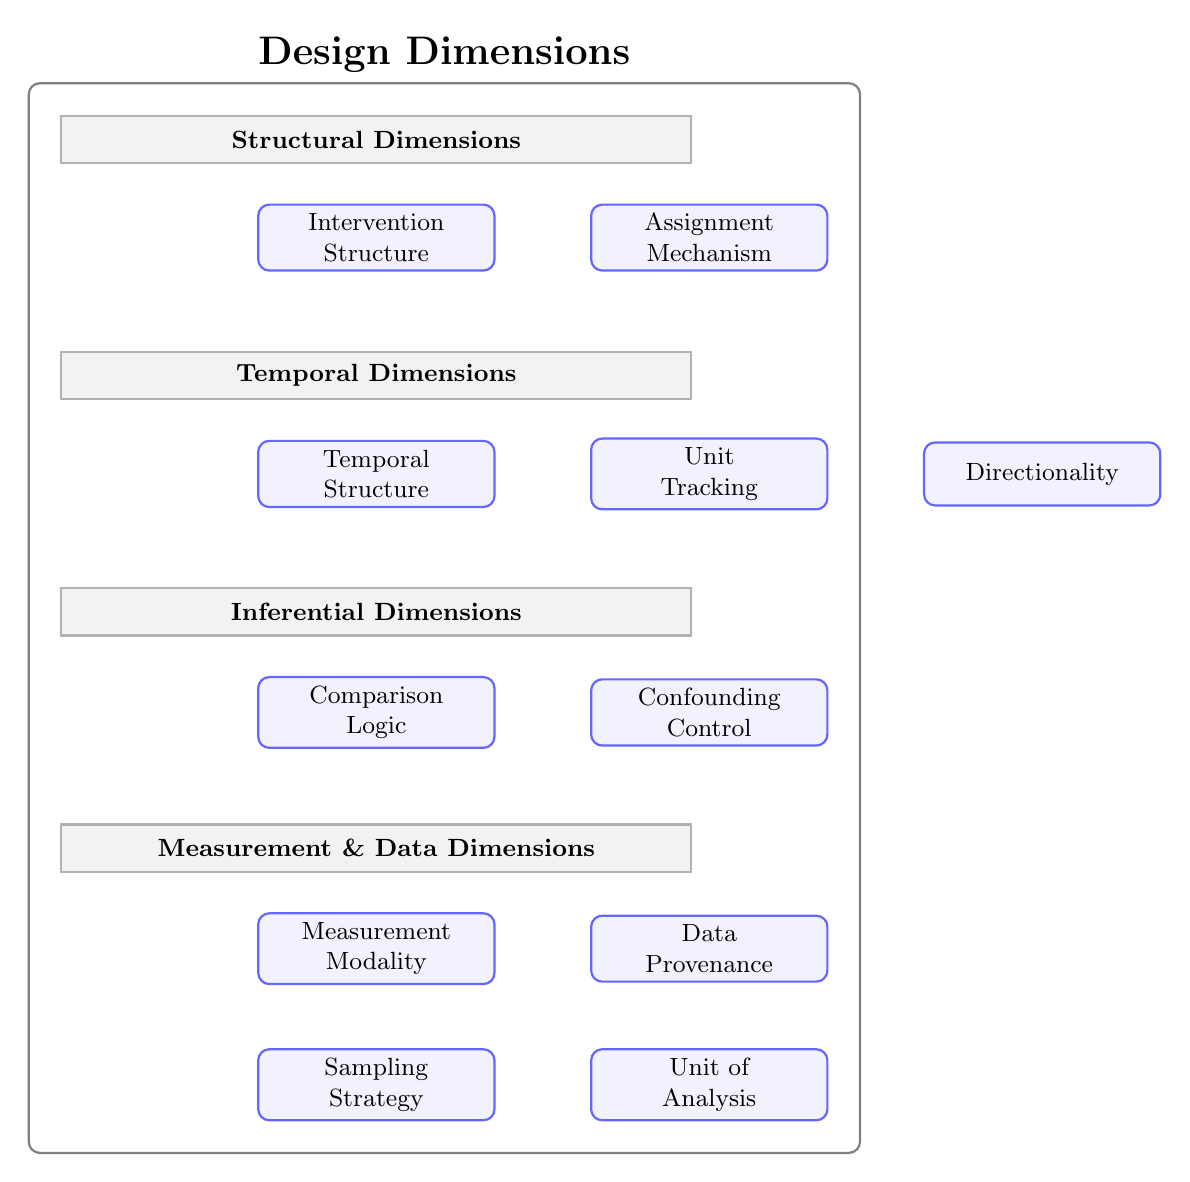
\begin{tikzpicture}[
    node distance=1.5cm and 1.2cm,
    dimension/.style={rectangle, rounded corners, draw=blue!60, fill=blue!5, thick, minimum width=3cm, minimum height=0.8cm, align=center, font=\small},
    category/.style={rectangle, draw=gray!60, fill=gray!10, thick, minimum width=8cm, minimum height=0.6cm, align=center, font=\small\bfseries},
]

% Category headers
\node[category] (structural) at (0,0) {Structural Dimensions};
\node[category] (temporal) at (0,-3) {Temporal Dimensions};
\node[category] (inference) at (0,-6) {Inferential Dimensions};
\node[category] (measurement) at (0,-9) {Measurement \& Data Dimensions};

% Structural dimensions
\node[dimension, below=0.5cm of structural] (intervention) {Intervention\\Structure};
\node[dimension, right=of intervention] (assignment) {Assignment\\Mechanism};

% Temporal dimensions
\node[dimension, below=0.5cm of temporal] (tempstruct) {Temporal\\Structure};
\node[dimension, right=of tempstruct] (tracking) {Unit\\Tracking};
\node[dimension, right=of tracking] (direction) {Directionality};

% Inferential dimensions
\node[dimension, below=0.5cm of inference] (comparison) {Comparison\\Logic};
\node[dimension, right=of comparison] (confounding) {Confounding\\Control};

% Measurement & data dimensions
\node[dimension, below=0.5cm of measurement] (measuremod) {Measurement\\Modality};
\node[dimension, right=of measuremod] (provenance) {Data\\Provenance};
\node[dimension, below=0.8cm of measuremod] (sampling) {Sampling\\Strategy};
\node[dimension, right=of sampling] (unitanalysis) {Unit of\\Analysis};

% Add a box around all dimensions
\node[draw=black!50, thick, rounded corners, fit=(structural) (intervention) (assignment) (unitanalysis) (sampling), inner sep=0.4cm, label=above:\Large\textbf{Design Dimensions}] (allbox) {};

\end{tikzpicture}
\caption{Taxonomy of Research Design Dimensions Organized by Conceptual Function}
\label{fig:dimensions-overview}
\end{figure}

% ============================================
% FIGURE 2: Dimension Interdependencies
% ============================================

\begin{figure}[htbp]
\centering
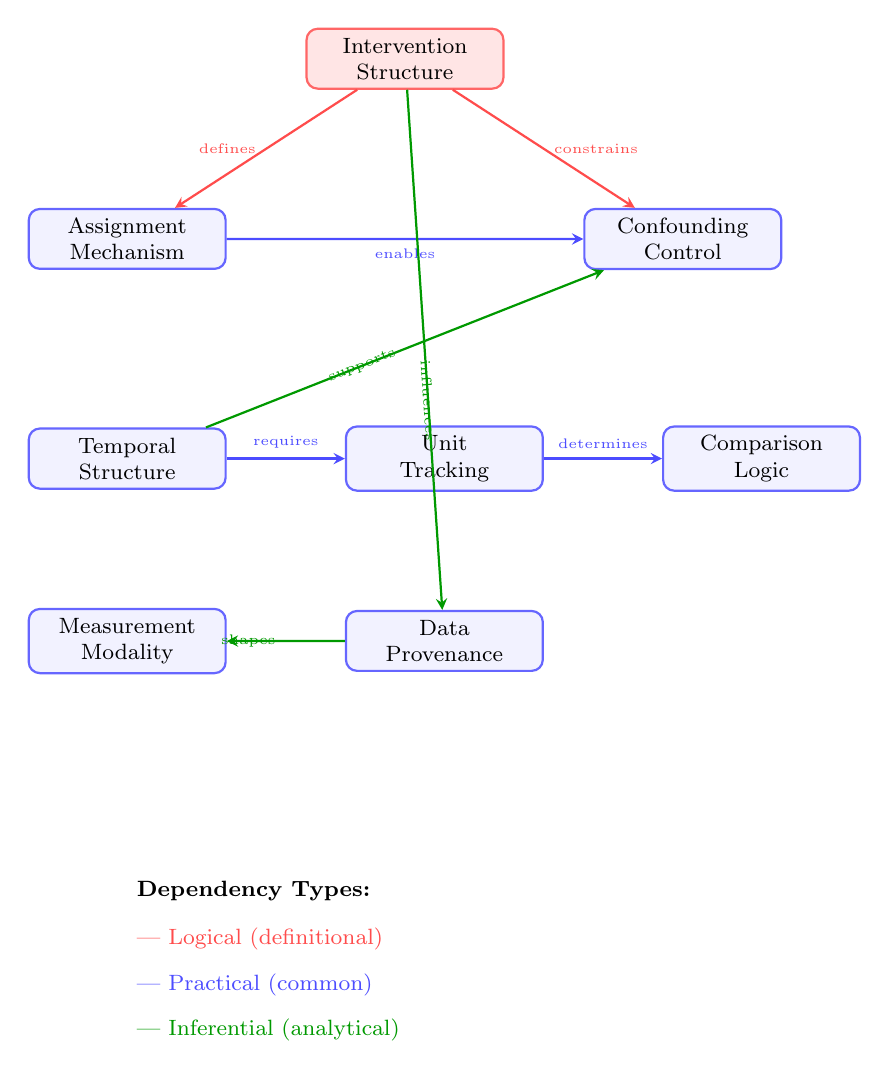
\begin{tikzpicture}[
    node distance=2cm and 1.5cm,
    dim/.style={rectangle, rounded corners, draw=blue!60, fill=blue!5, thick, minimum width=2.5cm, minimum height=0.7cm, align=center, font=\footnotesize},
    arrow/.style={->, >=stealth, thick},
]

% Core dimensions in a hierarchical layout
\node[dim, fill=red!10, draw=red!60] (intervention) {Intervention\\Structure};

\node[dim, below left=1.5cm and 1cm of intervention] (assignment) {Assignment\\Mechanism};
\node[dim, below right=1.5cm and 1cm of intervention] (confounding) {Confounding\\Control};

\node[dim, below=2cm of assignment] (temporal) {Temporal\\Structure};
\node[dim, right=1.5cm of temporal] (tracking) {Unit\\Tracking};
\node[dim, right=1.5cm of tracking] (comparison) {Comparison\\Logic};

\node[dim, below=1.5cm of temporal] (measurement) {Measurement\\Modality};
\node[dim, below=1.5cm of tracking] (provenance) {Data\\Provenance};

% Dependencies (logical and practical)
\draw[arrow, red!70] (intervention) -- (assignment) node[midway, left, font=\tiny] {defines};
\draw[arrow, red!70] (intervention) -- (confounding) node[midway, right, font=\tiny] {constrains};
\draw[arrow, blue!70] (assignment) -- (confounding) node[midway, below, font=\tiny, sloped] {enables};
\draw[arrow, blue!70] (temporal) -- (tracking) node[midway, above, font=\tiny] {requires};
\draw[arrow, blue!70] (tracking) -- (comparison) node[midway, above, font=\tiny] {determines};
\draw[arrow, green!60!black] (temporal) -- (confounding) node[midway, left, font=\tiny, sloped] {supports};
\draw[arrow, green!60!black] (intervention) -- (provenance) node[midway, right, font=\tiny, sloped] {influences};
\draw[arrow, green!60!black] (provenance) -- (measurement) node[midway, left, font=\tiny] {shapes};

% Legend - simplified without align option
\node[below=2.5cm of measurement, anchor=north west, font=\footnotesize] (legendtitle) {\textbf{Dependency Types:}};
\node[below=0.1cm of legendtitle.south west, anchor=north west, font=\footnotesize, text=red!70] (leg1) {--- Logical (definitional)};
\node[below=0.05cm of leg1.south west, anchor=north west, font=\footnotesize, text=blue!70] (leg2) {--- Practical (common)};
\node[below=0.05cm of leg2.south west, anchor=north west, font=\footnotesize, text=green!60!black] (leg3) {--- Inferential (analytical)};

\end{tikzpicture}
\caption{Key Interdependencies Among Design Dimensions}
\label{fig:dimension-dependencies}
\end{figure}

% ============================================
% FIGURE 3: Research Schemes Profiles (Simplified)
% ============================================

\begin{figure}[htbp]
\centering
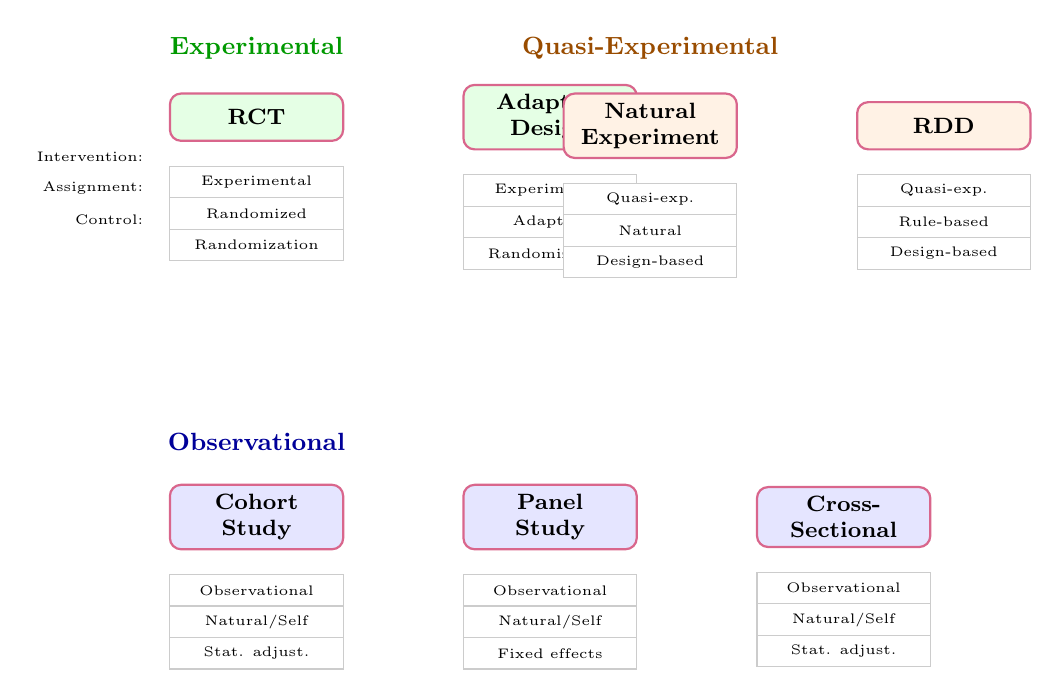
\begin{tikzpicture}[
    node distance=0.3cm,
    scheme/.style={rectangle, rounded corners, draw=purple!60, fill=purple!5, thick, minimum width=2.2cm, minimum height=0.6cm, align=center, font=\footnotesize\bfseries},
    dimvalue/.style={rectangle, draw=gray!40, fill=white, minimum width=2.2cm, minimum height=0.4cm, align=center, font=\tiny},
    dimlabel/.style={font=\tiny},
]

% Category labels at top
\node[font=\small, text=green!60!black] (exptitle) at (1,1) {\textbf{Experimental}};
\node[font=\small, text=orange!60!black] (quasititle) at (6,1) {\textbf{Quasi-Experimental}};
\node[font=\small, text=blue!60!black] (obstitle) at (1,-4) {\textbf{Observational}};

% Experimental Schemes
\node[scheme, fill=green!10, below=0.3cm of exptitle] (rct) {RCT};
\node[dimvalue, below=of rct] {Experimental};
\node[dimvalue, below=of rct, yshift=-0.4cm] {Randomized};
\node[dimvalue, below=of rct, yshift=-0.8cm] {Randomization};

\node[scheme, fill=green!10, right=1.5cm of rct] (adaptive) {Adaptive\\Design};
\node[dimvalue, below=of adaptive] {Experimental};
\node[dimvalue, below=of adaptive, yshift=-0.4cm] {Adaptive};
\node[dimvalue, below=of adaptive, yshift=-0.8cm] {Randomization};

% Quasi-experimental schemes
\node[scheme, fill=orange!10, below=0.3cm of quasititle] (natexp) {Natural\\Experiment};
\node[dimvalue, below=of natexp] {Quasi-exp.};
\node[dimvalue, below=of natexp, yshift=-0.4cm] {Natural};
\node[dimvalue, below=of natexp, yshift=-0.8cm] {Design-based};

\node[scheme, fill=orange!10, right=1.5cm of natexp] (rdd) {RDD};
\node[dimvalue, below=of rdd] {Quasi-exp.};
\node[dimvalue, below=of rdd, yshift=-0.4cm] {Rule-based};
\node[dimvalue, below=of rdd, yshift=-0.8cm] {Design-based};

% Observational schemes
\node[scheme, fill=blue!10, below=0.3cm of obstitle] (cohort) {Cohort\\Study};
\node[dimvalue, below=of cohort] {Observational};
\node[dimvalue, below=of cohort, yshift=-0.4cm] {Natural/Self};
\node[dimvalue, below=of cohort, yshift=-0.8cm] {Stat. adjust.};

\node[scheme, fill=blue!10, right=1.5cm of cohort] (panel) {Panel\\Study};
\node[dimvalue, below=of panel] {Observational};
\node[dimvalue, below=of panel, yshift=-0.4cm] {Natural/Self};
\node[dimvalue, below=of panel, yshift=-0.8cm] {Fixed effects};

\node[scheme, fill=blue!10, right=1.5cm of panel] (crosssect) {Cross-\\Sectional};
\node[dimvalue, below=of crosssect] {Observational};
\node[dimvalue, below=of crosssect, yshift=-0.4cm] {Natural/Self};
\node[dimvalue, below=of crosssect, yshift=-0.8cm] {Stat. adjust.};

% Dimension labels on left
\node[dimlabel, left=0.2cm of rct, yshift=-0.5cm] {Intervention:};
\node[dimlabel, left=0.2cm of rct, yshift=-0.9cm] {Assignment:};
\node[dimlabel, left=0.2cm of rct, yshift=-1.3cm] {Control:};

\end{tikzpicture}
\caption{Major Research Schemes and Their Dimensional Configurations}
\label{fig:schemes-profiles}
\end{figure}

% ============================================
% FIGURE 4: Design Space Navigation
% ============================================

\begin{figure}[htbp]
\centering
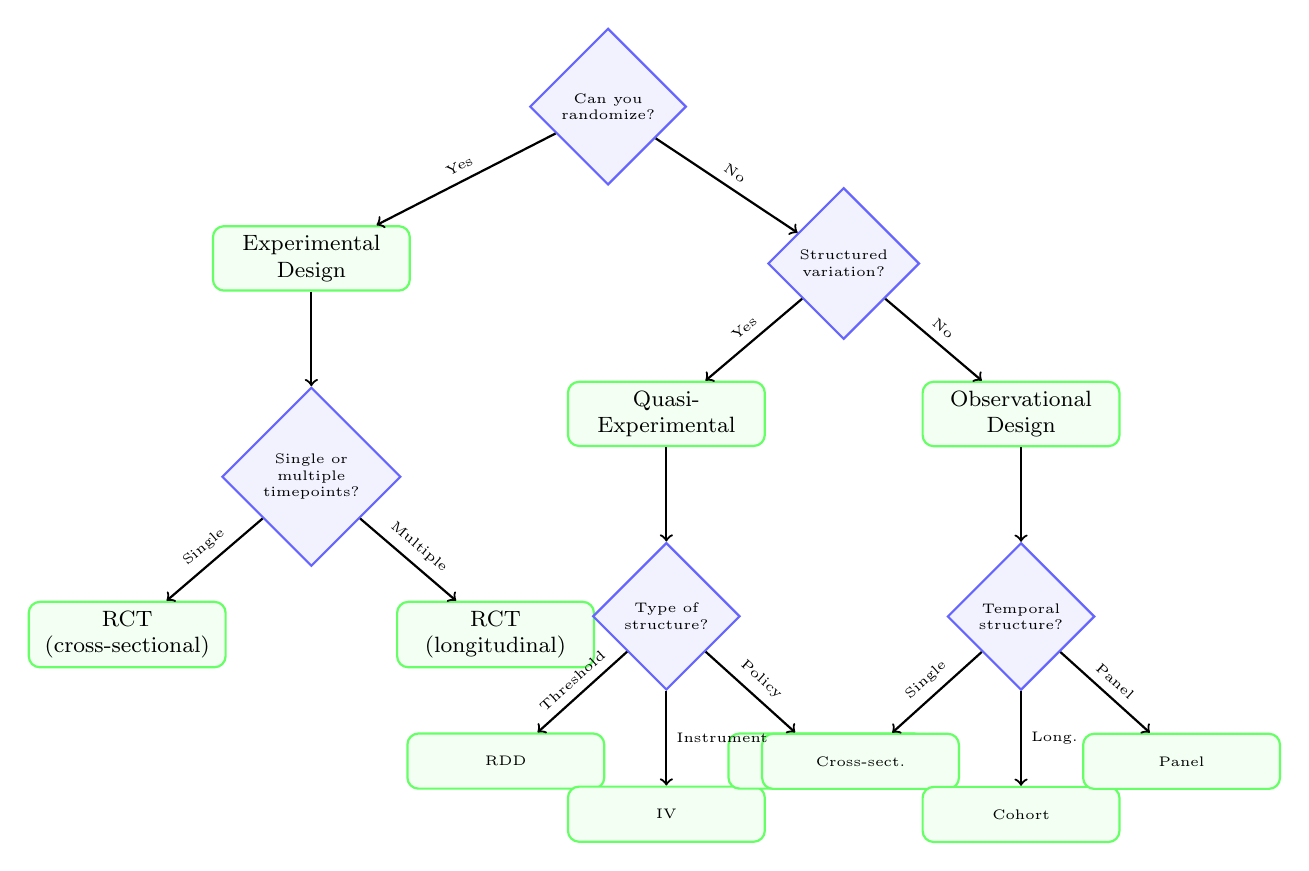
\begin{tikzpicture}[
    node distance=1.2cm,
    choice/.style={diamond, draw=blue!60, fill=blue!5, thick, minimum width=1.8cm, minimum height=1.2cm, align=center, font=\tiny},
    outcome/.style={rectangle, rounded corners, draw=green!60, fill=green!5, thick, minimum width=2.5cm, minimum height=0.7cm, align=center, font=\footnotesize},
]

% Starting point
\node[choice] (start) {Can you\\randomize?};

% Yes branch - Experimental
\node[outcome, below left=1cm and 2cm of start] (experimental) {Experimental\\Design};
\node[choice, below=of experimental] (exptemp) {Single or\\multiple\\timepoints?};
\node[outcome, below left=1cm and 0.5cm of exptemp] (rctcross) {RCT\\(cross-sectional)};
\node[outcome, below right=1cm and 0.5cm of exptemp] (rctlong) {RCT\\(longitudinal)};

% No branch - splits into quasi vs observational
\node[choice, below right=1cm and 2cm of start] (structured) {Structured\\variation?};

% Quasi-experimental branch
\node[outcome, below left=1cm and 0.5cm of structured] (quasi) {Quasi-\\Experimental};
\node[choice, below=of quasi] (quasitype) {Type of\\structure?};
\node[outcome, below left=1cm and 0.3cm of quasitype, font=\tiny] (rddout) {RDD};
\node[outcome, below=of quasitype, font=\tiny] (ivout) {IV};
\node[outcome, below right=1cm and 0.3cm of quasitype, font=\tiny] (didout) {DiD};

% Observational branch
\node[outcome, below right=1cm and 0.5cm of structured] (observational) {Observational\\Design};
\node[choice, below=of observational] (obstemp) {Temporal\\structure?};
\node[outcome, below left=1cm and 0.3cm of obstemp, font=\tiny] (cross) {Cross-sect.};
\node[outcome, below=of obstemp, font=\tiny] (cohortout) {Cohort};
\node[outcome, below right=1cm and 0.3cm of obstemp, font=\tiny] (panelout) {Panel};

% Arrows
\draw[->, thick] (start) -- (experimental) node[midway, above, sloped, font=\tiny] {Yes};
\draw[->, thick] (start) -- (structured) node[midway, above, sloped, font=\tiny] {No};
\draw[->, thick] (experimental) -- (exptemp);
\draw[->, thick] (exptemp) -- (rctcross) node[midway, above, sloped, font=\tiny] {Single};
\draw[->, thick] (exptemp) -- (rctlong) node[midway, above, sloped, font=\tiny] {Multiple};
\draw[->, thick] (structured) -- (quasi) node[midway, above, sloped, font=\tiny] {Yes};
\draw[->, thick] (structured) -- (observational) node[midway, above, sloped, font=\tiny] {No};
\draw[->, thick] (quasi) -- (quasitype);
\draw[->, thick] (quasitype) -- (rddout) node[midway, above, sloped, font=\tiny] {Threshold};
\draw[->, thick] (quasitype) -- (ivout) node[midway, right, font=\tiny] {Instrument};
\draw[->, thick] (quasitype) -- (didout) node[midway, above, sloped, font=\tiny] {Policy};
\draw[->, thick] (observational) -- (obstemp);
\draw[->, thick] (obstemp) -- (cross) node[midway, above, sloped, font=\tiny] {Single};
\draw[->, thick] (obstemp) -- (cohortout) node[midway, right, font=\tiny] {Long.};
\draw[->, thick] (obstemp) -- (panelout) node[midway, above, sloped, font=\tiny] {Panel};

\end{tikzpicture}
\caption{Design Space Navigation: How Key Dimensional Choices Lead to Canonical Research Schemes}
\label{fig:design-navigation}
\end{figure}

% ============================================
% FIGURE 5: Scheme-Dimension Matrix (SIMPLIFIED)
% ============================================

\begin{figure}[htbp]
\centering
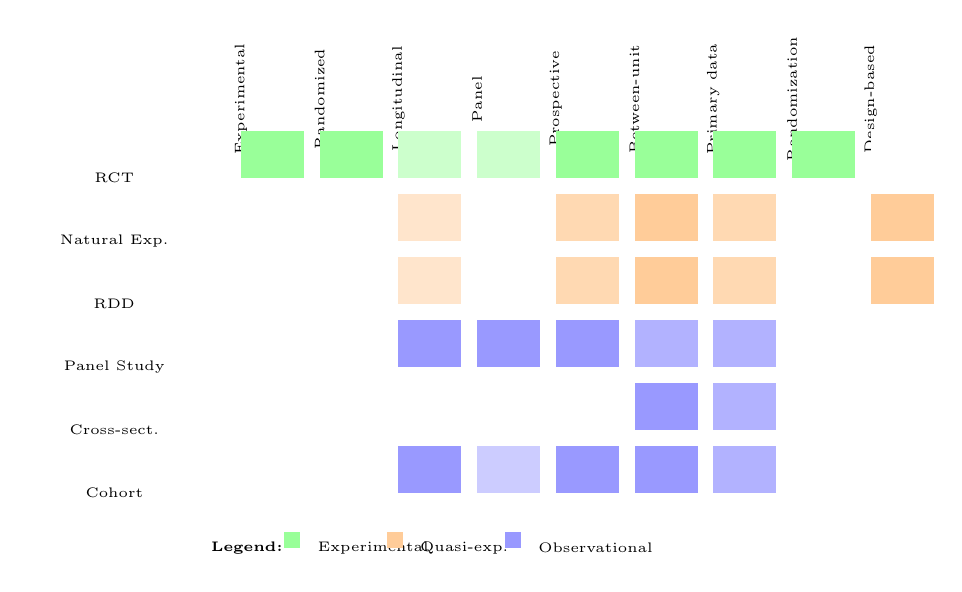
\begin{tikzpicture}[
    cell/.style={rectangle, minimum width=0.8cm, minimum height=0.6cm, draw=gray!30},
    header/.style={rectangle, minimum width=0.8cm, minimum height=0.6cm, font=\tiny},
    schemelabel/.style={rectangle, minimum width=2.2cm, minimum height=0.6cm, font=\tiny},
]

% Column headers (dimensions)
\node[header] at (0,0) {\rotatebox{90}{Experimental}};
\node[header] at (1,0) {\rotatebox{90}{Randomized}};
\node[header] at (2,0) {\rotatebox{90}{Longitudinal}};
\node[header] at (3,0) {\rotatebox{90}{Panel}};
\node[header] at (4,0) {\rotatebox{90}{Prospective}};
\node[header] at (5,0) {\rotatebox{90}{Between-unit}};
\node[header] at (6,0) {\rotatebox{90}{Primary data}};
\node[header] at (7,0) {\rotatebox{90}{Randomization}};
\node[header] at (8,0) {\rotatebox{90}{Design-based}};

% Schemes and their profiles
% RCT
\node[schemelabel, anchor=east] at (-0.5,-1) {RCT};
\fill[green!40] (0,-1) rectangle (0.8,-0.4);
\fill[green!40] (1,-1) rectangle (1.8,-0.4);
\fill[green!20] (2,-1) rectangle (2.8,-0.4);
\fill[green!20] (3,-1) rectangle (3.8,-0.4);
\fill[green!40] (4,-1) rectangle (4.8,-0.4);
\fill[green!40] (5,-1) rectangle (5.8,-0.4);
\fill[green!40] (6,-1) rectangle (6.8,-0.4);
\fill[green!40] (7,-1) rectangle (7.8,-0.4);
\fill[white] (8,-1) rectangle (8.8,-0.4);

% Natural Experiment
\node[schemelabel, anchor=east] at (-0.5,-1.8) {Natural Exp.};
\fill[white] (0,-1.8) rectangle (0.8,-1.2);
\fill[white] (1,-1.8) rectangle (1.8,-1.2);
\fill[orange!20] (2,-1.8) rectangle (2.8,-1.2);
\fill[white] (3,-1.8) rectangle (3.8,-1.2);
\fill[orange!30] (4,-1.8) rectangle (4.8,-1.2);
\fill[orange!40] (5,-1.8) rectangle (5.8,-1.2);
\fill[orange!30] (6,-1.8) rectangle (6.8,-1.2);
\fill[white] (7,-1.8) rectangle (7.8,-1.2);
\fill[orange!40] (8,-1.8) rectangle (8.8,-1.2);

% RDD
\node[schemelabel, anchor=east] at (-0.5,-2.6) {RDD};
\fill[white] (0,-2.6) rectangle (0.8,-2.0);
\fill[white] (1,-2.6) rectangle (1.8,-2.0);
\fill[orange!20] (2,-2.6) rectangle (2.8,-2.0);
\fill[white] (3,-2.6) rectangle (3.8,-2.0);
\fill[orange!30] (4,-2.6) rectangle (4.8,-2.0);
\fill[orange!40] (5,-2.6) rectangle (5.8,-2.0);
\fill[orange!30] (6,-2.6) rectangle (6.8,-2.0);
\fill[white] (7,-2.6) rectangle (7.8,-2.0);
\fill[orange!40] (8,-2.6) rectangle (8.8,-2.0);

% Panel Study
\node[schemelabel, anchor=east] at (-0.5,-3.4) {Panel Study};
\fill[white] (0,-3.4) rectangle (0.8,-2.8);
\fill[white] (1,-3.4) rectangle (1.8,-2.8);
\fill[blue!40] (2,-3.4) rectangle (2.8,-2.8);
\fill[blue!40] (3,-3.4) rectangle (3.8,-2.8);
\fill[blue!40] (4,-3.4) rectangle (4.8,-2.8);
\fill[blue!30] (5,-3.4) rectangle (5.8,-2.8);
\fill[blue!30] (6,-3.4) rectangle (6.8,-2.8);
\fill[white] (7,-3.4) rectangle (7.8,-2.8);
\fill[white] (8,-3.4) rectangle (8.8,-2.8);

% Cross-sectional
\node[schemelabel, anchor=east] at (-0.5,-4.2) {Cross-sect.};
\fill[white] (0,-4.2) rectangle (0.8,-3.6);
\fill[white] (1,-4.2) rectangle (1.8,-3.6);
\fill[white] (2,-4.2) rectangle (2.8,-3.6);
\fill[white] (3,-4.2) rectangle (3.8,-3.6);
\fill[white] (4,-4.2) rectangle (4.8,-3.6);
\fill[blue!40] (5,-4.2) rectangle (5.8,-3.6);
\fill[blue!30] (6,-4.2) rectangle (6.8,-3.6);
\fill[white] (7,-4.2) rectangle (7.8,-3.6);
\fill[white] (8,-4.2) rectangle (8.8,-3.6);

% Cohort Study
\node[schemelabel, anchor=east] at (-0.5,-5.0) {Cohort};
\fill[white] (0,-5.0) rectangle (0.8,-4.4);
\fill[white] (1,-5.0) rectangle (1.8,-4.4);
\fill[blue!40] (2,-5.0) rectangle (2.8,-4.4);
\fill[blue!20] (3,-5.0) rectangle (3.8,-4.4);
\fill[blue!40] (4,-5.0) rectangle (4.8,-4.4);
\fill[blue!40] (5,-5.0) rectangle (5.8,-4.4);
\fill[blue!30] (6,-5.0) rectangle (6.8,-4.4);
\fill[white] (7,-5.0) rectangle (7.8,-4.4);
\fill[white] (8,-5.0) rectangle (8.8,-4.4);

% Legend - completely simplified
\node[anchor=north west, font=\tiny] (lt) at (-0.5,-5.5) {\textbf{Legend:}};
\node[right=0.2cm of lt, font=\tiny] (leg1) {Experimental};
\fill[green!40] ([xshift=-0.3cm]leg1.west) rectangle ++(0.2,0.2);
\node[right=1.5cm of lt, font=\tiny] (leg2) {Quasi-exp.};
\fill[orange!40] ([xshift=-0.3cm]leg2.west) rectangle ++(0.2,0.2);
\node[right=3cm of lt, font=\tiny] (leg3) {Observational};
\fill[blue!40] ([xshift=-0.3cm]leg3.west) rectangle ++(0.2,0.2);

\end{tikzpicture}
\caption{Scheme-Dimension Matrix: Characteristic Values for Major Research Schemes}
\label{fig:scheme-dimension-matrix}
\end{figure}

% ============================================
% FIGURE 6: Conceptual Framework
% ============================================

\begin{figure}[htbp]
\centering
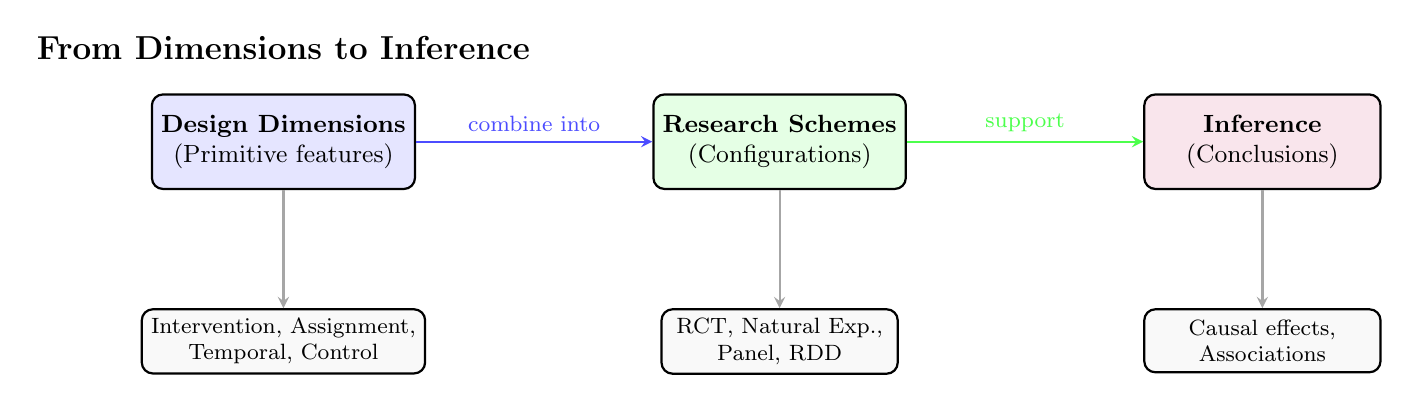
\begin{tikzpicture}[
    node distance=1.5cm,
    box/.style={rectangle, rounded corners, draw, thick, minimum width=3cm, minimum height=1.2cm, align=center, font=\small},
    arrow/.style={->, >=stealth, thick},
]

% Three main levels
\node[box, fill=blue!10] (dimensions) {\textbf{Design Dimensions}\\(Primitive features)};
\node[box, fill=green!10, right=3cm of dimensions] (schemes) {\textbf{Research Schemes}\\(Configurations)};
\node[box, fill=purple!10, right=3cm of schemes] (inference) {\textbf{Inference}\\(Conclusions)};

% Supporting elements
\node[box, fill=gray!5, below=1.5cm of dimensions, minimum height=0.8cm, font=\footnotesize, align=center] (dimexamples) {Intervention, Assignment,\\Temporal, Control};
\node[box, fill=gray!5, below=1.5cm of schemes, minimum height=0.8cm, font=\footnotesize, align=center] (schemeexamples) {RCT, Natural Exp.,\\Panel, RDD};
\node[box, fill=gray!5, below=1.5cm of inference, minimum height=0.8cm, font=\footnotesize, align=center] (inferenceexamples) {Causal effects,\\Associations};

% Arrows showing flow
\draw[arrow, blue!70] (dimensions) -- (schemes) node[midway, above, font=\footnotesize] {combine into};
\draw[arrow, green!70] (schemes) -- (inference) node[midway, above, font=\footnotesize] {support};
\draw[arrow, gray!70] (dimensions) -- (dimexamples);
\draw[arrow, gray!70] (schemes) -- (schemeexamples);
\draw[arrow, gray!70] (inference) -- (inferenceexamples);

% Title
\node[above=0.3cm of dimensions, font=\large\bfseries] {From Dimensions to Inference};

\end{tikzpicture}
\caption{Conceptual Framework: How Design Dimensions Combine into Research Schemes to Support Inference}
\label{fig:conceptual-framework}
\end{figure}

% ============================================
% FIGURE 7: Radial Layout of Dimensions
% ============================================

\begin{figure}[htbp]
\centering
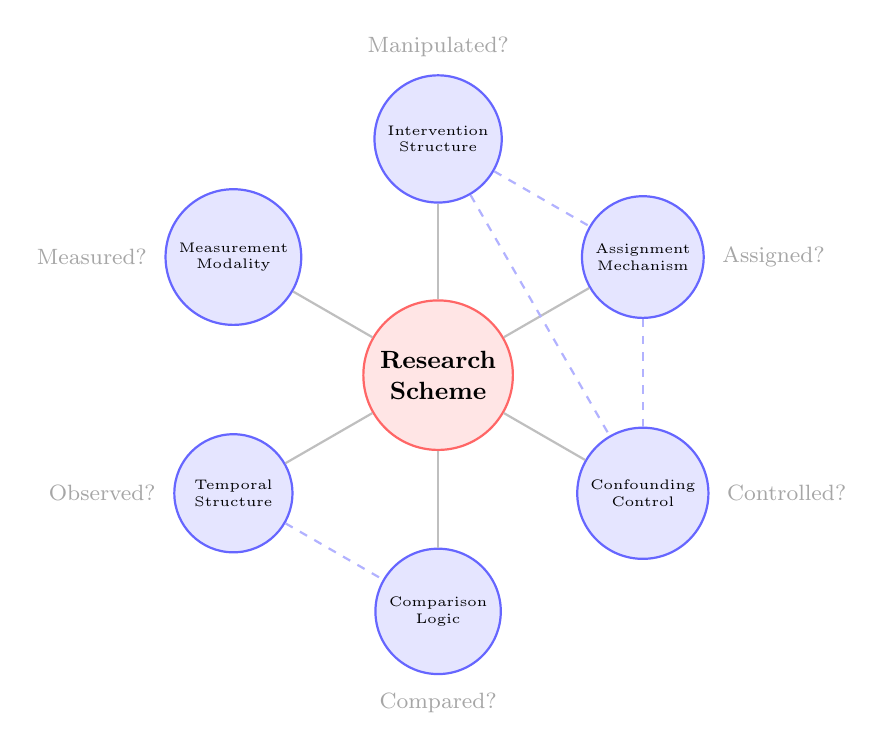
\begin{tikzpicture}[
    dim/.style={circle, draw=blue!60, fill=blue!10, thick, minimum size=1.5cm, align=center, font=\tiny},
    core/.style={circle, draw=red!60, fill=red!10, thick, minimum size=1.8cm, align=center, font=\small\bfseries},
]

% Central core
\node[core] (core) at (0,0) {Research\\Scheme};

% Dimensions arranged in circle
\node[dim] (intervention) at (0,3) {Intervention\\Structure};
\node[dim] (assignment) at (2.6,1.5) {Assignment\\Mechanism};
\node[dim] (confounding) at (2.6,-1.5) {Confounding\\Control};
\node[dim] (comparison) at (0,-3) {Comparison\\Logic};
\node[dim] (temporal) at (-2.6,-1.5) {Temporal\\Structure};
\node[dim] (measurement) at (-2.6,1.5) {Measurement\\Modality};

% Connections to core
\foreach \dim in {intervention, assignment, confounding, comparison, temporal, measurement} {
    \draw[thick, gray!50] (core) -- (\dim);
}

% Interdependencies between dimensions
\draw[thick, blue!30, dashed] (intervention) -- (assignment);
\draw[thick, blue!30, dashed] (assignment) -- (confounding);
\draw[thick, blue!30, dashed] (temporal) -- (comparison);
\draw[thick, blue!30, dashed] (intervention) -- (confounding);

% Outer labels
\node[font=\footnotesize, text=gray!70, above=0.1cm of intervention] {Manipulated?};
\node[font=\footnotesize, text=gray!70, right=0.1cm of assignment] {Assigned?};
\node[font=\footnotesize, text=gray!70, right=0.1cm of confounding] {Controlled?};
\node[font=\footnotesize, text=gray!70, below=0.1cm of comparison] {Compared?};
\node[font=\footnotesize, text=gray!70, left=0.1cm of temporal] {Observed?};
\node[font=\footnotesize, text=gray!70, left=0.1cm of measurement] {Measured?};

\end{tikzpicture}
\caption{Core Design Dimensions as an Interconnected System}
\label{fig:dimensions-radial}
\end{figure}

\section{Design Selection and Justification}

Selecting an appropriate research design involves mapping the research question to a feasible and inferentially defensible configuration of design dimensions. This process requires:

\begin{enumerate}
    \item \textbf{Clarifying the inferential goal}: Is the objective causal identification, descriptive characterization, prediction, or hypothesis generation? What population and effect are of interest?
    
    \item \textbf{Identifying constraints}: What ethical, practical, temporal, or resource constraints limit design options? Are randomization or experimental manipulation feasible? What measurement modalities are available and valid for key constructs?
    
    \item \textbf{Assessing identification strategies}: What assumptions are required for valid inference under each feasible design? Which confounding control strategies are available given the data structure?
    
    \item \textbf{Evaluating tradeoffs}: How do different designs balance internal validity, external validity, precision, bias, measurement validity, and ethical considerations?
    
    \item \textbf{Justifying the chosen design}: Explicitly articulate why the selected configuration is appropriate given the research context, what assumptions it relies upon, and why alternative configurations are less suitable.
\end{enumerate}

Design justification is not merely procedural. It requires substantive argumentation about why the chosen dimensional configuration supports the intended inference and why alternative configurations are less suitable. This justification should address both the strengths and limitations of the design, including the assumptions on which valid inference depends.

\subsection{Design Justification Template}

A complete design justification should address:

\begin{itemize}
    \item \textbf{Research question and inferential goal}: What is the target estimand? Is causal identification required?
    
    \item \textbf{Intervention structure justification}: Why is the chosen level of intervention (experimental, quasi-experimental, observational) appropriate or necessary?
    
    \item \textbf{Assignment mechanism rationale}: How does the assignment mechanism support or constrain causal inference?
    
    \item \textbf{Temporal design rationale}: Why is the chosen temporal structure sufficient for the research question?
    
    \item \textbf{Measurement validity argument}: Why are the chosen measurement modalities valid for the constructs of interest? What are their known biases and how are they addressed?
    
    \item \textbf{Confounding control justification}: What confounding control strategy is employed? What assumptions does it require? Why are these assumptions plausible in this context? What sensitivity analyses or robustness checks are conducted?
    
    \item \textbf{Alternative designs considered}: What other dimensional configurations were considered? Why were they rejected (infeasibility, ethical concerns, weaker identification)?
    
    \item \textbf{Limitations acknowledged}: What are the key limitations of the chosen design? What threats to validity remain? How might these limitations affect interpretation?
\end{itemize}

Transparent articulation of design logic strengthens the credibility of empirical claims and enables critical evaluation by the scientific community.

\subsection{Example: Design Justification for a Cohort Study of Educational Interventions}

\emph{Research question}: Does participation in an afterschool mentoring program improve high school graduation rates among at-risk youth?

\emph{Dimensional configuration}: Observational design with self-selection into mentoring; longitudinal temporal structure following students from program entry through graduation-eligible age; cohort tracking of students who entered high school in the same year; prospective directionality with program participation measured at baseline and graduation observed subsequently; between-unit comparison of program participants and non-participants; primary data collection through surveys and administrative records; statistical adjustment using propensity score weighting to control confounding.

\emph{Justification}: 
\begin{itemize}
    \item Random assignment to mentoring is infeasible because the program operates outside researcher control and denying mentoring to willing participants raises ethical concerns.
    \item Longitudinal temporal structure is necessary to establish temporal precedence and observe graduation outcomes, which occur years after program entry.
    \item Cohort design ensures comparability in terms of entry year, reducing confounding by cohort-specific factors (e.g., policy changes, economic conditions).
    \item Prospective directionality minimizes recall bias in program participation measurement.
    \item Propensity score weighting controls for observed confounders (prior academic performance, socioeconomic status, family structure, neighborhood characteristics) that predict both program participation and graduation. Conditional independence is plausible if all key confounders are measured.
    \item Administrative records for graduation outcomes reduce measurement error relative to self-report.
    \item Limitations: Unmeasured confounding remains possible (e.g., student motivation, family support). Sensitivity analyses quantify the strength of unmeasured confounding needed to eliminate the observed effect. External validity is limited to the specific program and student population studied.
\end{itemize}

This justification explicates the logic linking design choices to inferential goals, acknowledges assumptions and limitations, and demonstrates considered decision-making. 

\section{Recap: From Research Questions to Research Schemes}

The relationship between research questions and research schemes is not mechanical. Researchers do not simply "apply" a predetermined scheme to a given question. Instead, design selection emerges from an iterative process of conceptualization, operationalization, and constraint mapping. This section describes the practical workflow through which researchers move from substantive questions to feasible research designs.

\subsection{The Design Selection Workflow}

Research design begins with a substantive question and proceeds through several stages of refinement and constraint assessment. The process is rarely linear—researchers often cycle between stages as they discover new constraints or refine their understanding of what is feasible and inferentially defensible.

\subsubsection{Stage 1: Conceptual Clarification}

Before selecting a design, researchers must clarify what they are trying to learn. This involves:

\paragraph{Articulating the substantive question.} What real-world phenomenon or relationship are you trying to understand? For example: "Do afterschool programs improve academic outcomes?" or "How does social media use affect mental health?"

\paragraph{Identifying the type of inference desired.} Different research goals require different designs:
\begin{itemize}
    \item \emph{Causal inference}: Estimating the effect of an intervention or exposure on an outcome (e.g., "Does X cause Y?")
    \item \emph{Descriptive inference}: Characterizing a population, distribution, or relationship (e.g., "What proportion of X exhibit Y?")
    \item \emph{Predictive inference}: Forecasting future outcomes or states (e.g., "Given X, what is the likely value of Y?")
    \item \emph{Exploratory inquiry}: Generating hypotheses or identifying patterns (e.g., "What factors are associated with Y?")
\end{itemize}

The inferential goal fundamentally constrains design options. Causal inference requires temporal precedence and confounding control. Descriptive inference may not require these features but demands representative sampling. Prediction prioritizes out-of-sample performance over causal interpretation.

\paragraph{Defining the target population and estimand.} For whom or what should the inference hold? The target population determines sampling requirements. The estimand (the quantity to be estimated) determines what comparisons must be constructed and what variation must be observed.

\subsubsection{Stage 2: Operationalization}

Conceptual clarity must be translated into measurable variables and observable units. This stage involves:

\paragraph{Defining units of observation and analysis.} What are the entities being studied? Individuals? Organizations? Geographic areas? Time periods? The unit definition affects what data sources are available and what level of aggregation is appropriate.

\paragraph{Operationalizing key constructs.} How will abstract concepts (e.g., "program participation," "academic achievement," "mental health") be measured? Available measurement modalities constrain design options. If valid biomarkers exist, experimental designs with objective measurement become more feasible. If only self-report is available, designs must account for reporting bias.

\paragraph{Identifying the exposure or treatment of interest.} What is the intervention, exposure, or predictor whose effect or association is of interest? Can it be manipulated? Is it binary or continuous? Does it vary naturally? These characteristics determine whether experimental, quasi-experimental, or observational designs are possible.

\paragraph{Specifying the outcome.} What is being affected or predicted? When can it be observed? How long after exposure does it occur? The temporal gap between exposure and outcome determines the required duration of follow-up and whether prospective or retrospective observation is feasible.

At this stage, researchers often discover that their initial question is not operationalizable with available measures. This may require reconceptualizing the question, seeking new measurement tools, or accepting that some aspects of the question cannot be empirically addressed.

\subsubsection{Stage 3: Constraint Assessment}

With a clear question and operational definitions, researchers assess what designs are feasible given practical, ethical, and resource constraints:

\paragraph{Ethical constraints.} Can the exposure be manipulated? Is random assignment ethically acceptable? Harmful exposures cannot be experimentally assigned. Withholding beneficial interventions from control groups may be unethical. These constraints rule out certain experimental designs.

\paragraph{Feasibility constraints.} Can the researcher control assignment? Do the necessary data exist? Can subjects be followed over time? Many exposures (race, gender, early-life experiences) cannot be manipulated. Many outcomes (rare diseases, long-term effects) cannot be observed within typical research timelines. These constraints often necessitate observational designs.

\paragraph{Resource constraints.} What is affordable in terms of time, funding, and personnel? Experimental designs with primary data collection are expensive. Longitudinal designs require sustained funding. Large representative samples are costly. Resource constraints may force compromises between ideal and feasible designs.

\paragraph{Temporal constraints.} How quickly are results needed? Experimental trials require time for recruitment, intervention, and follow-up. Longitudinal designs span years or decades. Secondary data analysis can be rapid but sacrifices control over measurement. Urgent questions may necessitate cross-sectional designs despite inferential limitations.

\paragraph{Data availability.} What data already exist? Administrative records may enable large-scale quasi-experimental designs at low cost but with construct validity concerns. Survey data may provide rich measurement but limited sample sizes. The existence and accessibility of secondary data fundamentally shapes design options.

Constraint assessment often reveals that the ideal design for the research question is infeasible. This forces researchers to select among imperfect alternatives, balancing inferential strength against practical realities.

\subsubsection{Stage 4: Dimensional Configuration}

Given the clarified question and assessed constraints, researchers now configure design dimensions to construct a feasible scheme:

\paragraph{Intervention structure.} If manipulation is ethical and feasible, experimental designs are possible. If manipulation is impossible but structured natural variation exists (policy changes, thresholds, instruments), quasi-experimental designs may be viable. Otherwise, observational designs are necessary.

\paragraph{Assignment mechanism.} If intervention is possible, can randomization be implemented? If not, what determines assignment? The assignment mechanism determines what identification strategies are available and what assumptions must be invoked.

\paragraph{Temporal structure and unit tracking.} Can units be followed over time? Is repeated observation feasible given attrition and cost? The temporal dimension is determined by the need to establish temporal precedence, observe change, or exploit within-unit variation for confounding control.

\paragraph{Comparison logic.} What source of counterfactual comparison is most credible? Between-unit comparisons require exchangeability (achieved through randomization, matching, or adjustment). Within-unit comparisons require temporal stability. The comparison logic follows from the assignment mechanism and available data.

\paragraph{Confounding control strategy.} Given the assignment mechanism, temporal structure, and available covariates, what confounding control is possible? Randomization eliminates confounding by design. Design-based identification (RDD, IV, DiD) exploits structural features. Statistical adjustment relies on measured confounders. The control strategy is constrained by prior dimensional choices.

\paragraph{Measurement modality and data provenance.} What measurement approaches are valid and feasible for key constructs? Primary data allow tailored measurement but at high cost. Secondary data are cheaper but may not align well with constructs. The measurement dimension is constrained by budget, construct definitions, and data availability.

This configuration process is iterative: choices on one dimension constrain options on others. For example, choosing longitudinal temporal structure enables fixed effects confounding control, which in turn may reduce the need for rich covariate measurement. Researchers navigate this constrained design space, seeking coherent configurations that support the intended inference.

\subsubsection{Stage 5: Scheme Recognition and Adaptation}

Once dimensional values are configured, researchers often recognize that their design corresponds to a canonical research scheme. This recognition is valuable because schemes come with established inferential frameworks, known assumptions, and standard methods.

For example, a design with:
\begin{itemize}
    \item Observational intervention
    \item Self-selection assignment
    \item Longitudinal temporal structure
    \item Cohort tracking
    \item Prospective directionality
    \item Between-unit comparison
    \item Primary data
    \item Statistical adjustment for confounding
\end{itemize}
is recognizable as a \emph{cohort study}. This recognition connects the design to a literature on cohort study methods, standard analysis approaches, and typical threats to validity.

However, many real designs do not perfectly match canonical schemes. Researchers may combine features from multiple schemes or create hybrid designs tailored to specific contexts. The dimensional framework enables precise communication about such designs even when they do not fit standard categories.

\subsection{Justifying Design Choices}

Design justification articulates the logic connecting research question, constraints, dimensional configuration, and inferential assumptions. A complete justification addresses:

\paragraph{Why this inferential goal?} What substantive question motivates the study? What type of inference (causal, descriptive, predictive) is required to address it?

\paragraph{Why these operational definitions?} How do the chosen measures capture the constructs of interest? What measurement biases exist and how are they addressed or acknowledged?

\paragraph{Why this dimensional configuration?} For each dimension, explain:
\begin{itemize}
    \item What alternatives were considered
    \item What constraints ruled them out or made them less desirable
    \item How the chosen value supports the inferential goal
\end{itemize}

\paragraph{What assumptions does this design require?} Make explicit the identifying assumptions on which valid inference depends. For example:
\begin{itemize}
    \item Experimental designs assume compliance and no spillover
    \item Quasi-experimental designs have design-specific assumptions (parallel trends for DiD, continuity for RDD, exclusion restriction for IV)
    \item Observational designs with statistical adjustment assume conditional independence (no unmeasured confounding)
\end{itemize}

\paragraph{How plausible are these assumptions?} Provide substantive arguments or empirical evidence supporting key assumptions. Discuss what would have to be true for assumptions to be violated and whether such violations seem likely.

\paragraph{What are the key limitations?} Acknowledge what the design cannot do. What threats to validity remain unaddressed? How might violations of assumptions or other limitations affect interpretation?

\paragraph{What sensitivity analyses are planned?} How will robustness of findings to assumption violations be assessed? For observational designs, how strong would unmeasured confounding need to be to overturn results?

\subsection{Example: From Question to Design}

To illustrate the workflow, consider the development of a study design for the question: "Does participation in afterschool mentoring programs improve high school graduation rates among at-risk youth?"

\paragraph{Stage 1: Conceptual clarification.}
\begin{itemize}
    \item Inferential goal: Causal inference (effect of mentoring on graduation)
    \item Target population: At-risk youth (operationally defined as students with low prior achievement or socioeconomic disadvantage)
    \item Estimand: Average treatment effect of mentoring participation on graduation probability
\end{itemize}

\paragraph{Stage 2: Operationalization.}
\begin{itemize}
    \item Units: Individual students
    \item Exposure: Participation in specific mentoring program (binary: participant vs. non-participant)
    \item Outcome: High school graduation (binary: graduate vs. not), observed 4-5 years after program entry
    \item Key covariates: Prior academic performance, socioeconomic status, family structure, neighborhood characteristics (available from school records and baseline survey)
\end{itemize}

\paragraph{Stage 3: Constraint assessment.}
\begin{itemize}
    \item Ethical constraints: Random assignment infeasible—program operates independently and denying mentoring to willing students is ethically problematic
    \item Feasibility: Cannot manipulate program participation; program enrollment is voluntary
    \item Resources: Moderate budget allows baseline survey and administrative data linkage but not intensive primary data collection
    \item Temporal: Results needed within 6 years; graduation outcomes observable within this window
    \item Data: Administrative graduation records available; baseline survey feasible; no biomarkers needed
\end{itemize}

\paragraph{Stage 4: Dimensional configuration.}
\begin{itemize}
    \item Intervention: Observational (cannot randomize)
    \item Assignment: Self-selection (students choose whether to participate)
    \item Temporal: Longitudinal (must follow students from program entry to graduation)
    \item Unit tracking: Cohort (follow students entering high school in same year to control cohort effects)
    \item Directionality: Prospective (measure participation at baseline, observe graduation later)
    \item Comparison: Between-unit (compare participants to non-participants)
    \item Data provenance: Mixed (baseline survey + administrative graduation records)
    \item Measurement: Self-report for participation, administrative records for graduation
    \item Confounding control: Statistical adjustment via propensity score weighting (observed confounders predict both participation and graduation)
\end{itemize}

\paragraph{Stage 5: Scheme recognition.}
This configuration is recognizable as a prospective cohort study with propensity score adjustment. The design follows established cohort study methods while adapting to the specific context (mentoring programs, educational outcomes).

\paragraph{Justification.}
\begin{itemize}
    \item Random assignment ruled out by ethical and feasibility constraints
    \item Longitudinal structure necessary to observe graduation outcomes and establish temporal precedence
    \item Cohort design controls for cohort-specific confounders (policy changes, economic conditions)
    \item Propensity score weighting addresses selection bias by balancing groups on observed characteristics
    \item Key assumption: Conditional independence—all important confounders measured (plausible given rich administrative data and baseline survey)
    \item Limitations: Unmeasured confounding possible (e.g., student motivation, family support not fully captured). Sensitivity analyses will quantify robustness to unmeasured confounding. External validity limited to this program and population.
\end{itemize}

This example shows how design selection proceeds from question to constraints to dimensional configuration to scheme recognition, with justification explaining the logic at each step.

\subsection{Common Design Selection Patterns}

Certain patterns recur in design selection workflows. Recognizing these patterns helps researchers navigate the design space more efficiently.

\paragraph{Pattern 1: Ideal design infeasible → closest feasible alternative.}
Researchers often begin with an ideal design (typically an RCT for causal questions) but discover it is infeasible. The task becomes finding the closest approximation that remains feasible. This might mean:
\begin{itemize}
    \item Experimental → Quasi-experimental (exploiting natural experiments, RDD, or IV when randomization is impossible)
    \item Randomized → Matching/adjustment (when assignment cannot be controlled but rich covariates are available)
    \item Longitudinal → Cross-sectional (when follow-up is impossible, accepting limitations on temporal inference)
\end{itemize}

\paragraph{Pattern 2: Constraint-driven dimension fixing.}
Some constraints directly determine dimensional values, which then cascade to constrain other dimensions:
\begin{itemize}
    \item Cannot manipulate exposure → Observational intervention → Self-selection or natural assignment → Need confounding control through matching/adjustment or design-based identification
    \item Cannot follow units over time → Cross-sectional temporal structure → Cannot use within-unit comparison or fixed effects → Must rely on between-unit comparisons
    \item Only secondary data available → Predetermined measurement modality and data provenance → Construct validity concerns → May need validation studies
\end{itemize}

\paragraph{Pattern 3: Opportunistic design.}
Sometimes researchers discover unexpected opportunities that enable stronger designs:
\begin{itemize}
    \item Policy change creates natural experiment enabling DiD or synthetic control
    \item Threshold-based program eligibility enables RDD
    \item Lottery-based oversubscribed program enables IV design
    \item Existing high-quality administrative data enables large-scale observational analysis
\end{itemize}
Opportunistic designs require recognizing these structural features and adapting methods to exploit them.

\paragraph{Pattern 4: Hybrid and adaptive designs.}
Researchers increasingly combine features from multiple canonical schemes:
\begin{itemize}
    \item RDD with difference-in-differences (exploiting both threshold and panel structure)
    \item Matching combined with regression adjustment (doubly robust estimation)
    \item Natural experiment with synthetic controls (for improved comparison group construction)
    \item Experimental design with administrative data linkage (reducing measurement cost and attrition)
\end{itemize}

These patterns reflect the reality that design selection is a pragmatic problem-solving process, not a formulaic application of standard templates.

\subsection{Moving Forward: Design to Analysis}

Once a research scheme is selected and justified, researchers proceed to:
\begin{itemize}
    \item Specifying the statistical model or estimation strategy appropriate for the scheme
    \item Determining sample size and power requirements
    \item Developing data collection protocols (for primary data) or data access strategies (for secondary data)
    \item Planning sensitivity analyses and robustness checks
    \item Anticipating and planning for threats to validity specific to the chosen design
\end{itemize}

These implementation details build on the dimensional configuration established during design selection. The dimensional framework provides the conceptual foundation; subsequent chapters on estimation, inference, and validity build the technical superstructure.

The key insight is that research design is not a matter of selecting a pre-packaged scheme from a menu. It is a process of navigating a constrained design space, configuring dimensions to balance inferential goals against practical realities, and justifying the resulting configuration through transparent articulation of assumptions and limitations.


\section{Case Studies: Research Schemes in Practice}

This section presents real-world examples of canonical research schemes, illustrating how dimensional configurations are realized in actual studies. Each case study identifies the research question, dimensional configuration, key design features, and main findings, demonstrating how abstract design principles translate into concrete empirical work.

\subsection{Randomized Controlled Trials}

\subsubsection{Case Study 1: Moving to Opportunity Experiment}

\paragraph{Research Question.} Does moving from high-poverty to low-poverty neighborhoods improve economic and health outcomes for families?

\paragraph{Background.} The Moving to Opportunity (MTO) experiment, conducted by the U.S. Department of Housing and Urban Development from 1994-1998, examined whether residential mobility could improve outcomes for families living in public housing in high-poverty neighborhoods.

\paragraph{Dimensional Configuration.}
\begin{itemize}
    \item \textbf{Intervention}: Experimental (researchers controlled housing voucher assignment)
    \item \textbf{Assignment}: Randomized (lottery-based assignment to three groups)
    \item \textbf{Temporal}: Longitudinal (followed families for 10-15 years)
    \item \textbf{Unit tracking}: Panel (same families tracked over time)
    \item \textbf{Directionality}: Prospective (voucher assignment preceded outcome measurement)
    \item \textbf{Comparison}: Between-unit (experimental vs. control groups)
    \item \textbf{Data provenance}: Mixed (baseline surveys, administrative records, follow-up surveys)
    \item \textbf{Measurement}: Administrative records (earnings, education), surveys (health, well-being), direct assessment (children's achievement tests)
    \item \textbf{Confounding control}: Randomization-based
\end{itemize}

\paragraph{Key Design Features.}
\begin{itemize}
    \item 4,604 low-income families with children randomized to: (1) experimental voucher (must move to low-poverty area), (2) Section 8 voucher (no location restriction), or (3) control (no voucher)
    \item Compliance issues: Not all families assigned vouchers used them; not all experimental group families moved to low-poverty areas
    \item Long-term follow-up enabled assessment of effects on children who were young at randomization
\end{itemize}

\paragraph{Key Findings.} Moving to lower-poverty neighborhoods produced mixed results: improved mental health and subjective well-being for adults, reduced obesity and diabetes, but little effect on economic self-sufficiency. For children, effects depended critically on age at move: children who moved before age 13 had substantially higher earnings as adults, while those who moved as adolescents showed no earnings gains.

\paragraph{Lessons.} This case illustrates: (1) the power of randomization to answer causal questions that would be confounded in observational studies (families who voluntarily move differ from those who don't), (2) the importance of long-term follow-up for outcomes that take years to manifest, (3) compliance challenges even in experimental designs, and (4) the value of examining heterogeneous treatment effects by subgroup (age at move).

\subsubsection{Case Study 2: Oregon Health Insurance Experiment}

\paragraph{Research Question.} What is the causal effect of health insurance coverage on health outcomes and healthcare utilization?

\paragraph{Background.} In 2008, Oregon expanded its Medicaid program through a lottery due to budget constraints, creating a rare opportunity for a randomized evaluation of health insurance.

\paragraph{Dimensional Configuration.}
\begin{itemize}
    \item \textbf{Intervention}: Experimental (lottery-based selection for Medicaid)
    \item \textbf{Assignment}: Randomized (lottery determined eligibility)
    \item \textbf{Temporal}: Longitudinal (baseline and follow-up measurements)
    \item \textbf{Comparison}: Between-unit (lottery winners vs. losers)
    \item \textbf{Data provenance}: Mixed (administrative hospital records, credit reports, in-person health assessments, surveys)
    \item \textbf{Measurement}: Biomarkers (blood pressure, cholesterol, blood sugar), administrative records (hospital visits, credit), self-report (health status, access)
    \item \textbf{Confounding control}: Randomization via lottery
\end{itemize}

\paragraph{Key Findings.} Medicaid coverage increased healthcare utilization, reduced financial strain (fewer medical debts), and improved self-reported health and mental health. However, no statistically significant effects were detected on measured physical health outcomes (blood pressure, cholesterol, glycated hemoglobin) after two years, though confidence intervals included clinically meaningful effects.

\paragraph{Lessons.} Natural policy variation can create experimental opportunities. Biomarker measurement provided objective health assessment beyond self-report. The null findings on some outcomes were scientifically valuable, demonstrating that causal effects may differ from observational associations.

\subsection{Quasi-Experimental Designs}

\subsubsection{Case Study 3: Minimum Wage and Employment (Card \& Krueger)}

\paragraph{Research Question.} Does raising the minimum wage reduce employment, as predicted by standard economic theory?

\paragraph{Background.} In 1992, New Jersey raised its minimum wage from \$4.25 to \$5.05 while neighboring Pennsylvania's minimum wage remained unchanged, creating a natural experiment.

\paragraph{Dimensional Configuration.}
\begin{itemize}
    \item \textbf{Intervention}: Quasi-experimental (policy change not controlled by researchers)
    \item \textbf{Assignment}: Natural (state-level policy determined exposure)
    \item \textbf{Temporal}: Longitudinal (before and after wage increase)
    \item \textbf{Comparison}: Between-unit (NJ vs. PA) and within-unit (same restaurants before/after)
    \item \textbf{Data provenance}: Primary (telephone surveys of fast-food restaurants)
    \item \textbf{Confounding control}: Design-based (difference-in-differences)
\end{itemize}

\paragraph{Key Design Features.}
\begin{itemize}
    \item Difference-in-differences design: compared change in employment in NJ (treatment) to change in PA (control)
    \item Parallel trends assumption: NJ and PA would have followed similar employment trends absent the wage increase
    \item Focus on fast-food industry where minimum wage workers are concentrated
\end{itemize}

\paragraph{Key Findings.} Contrary to standard predictions, employment in NJ fast-food restaurants increased slightly relative to PA following the wage increase. No evidence that minimum wage increase reduced employment.

\paragraph{Lessons.} Natural policy variation can enable causal inference when randomization is impossible. DiD design controls for state-specific time-invariant factors and common time trends. Geographic comparison units (neighboring states) increase plausibility of parallel trends. Findings challenged conventional wisdom and sparked extensive methodological and substantive debate.

\subsubsection{Case Study 4: Class Size and Achievement (Angrist \& Lavy, RDD)}

\paragraph{Research Question.} Does reducing class size improve student achievement?

\paragraph{Background.} Israeli schools follow a rule limiting class size to 40 students (Maimonides' rule). When enrollment exceeds 40, schools must create two classes, creating sharp discontinuities in class size at enrollment thresholds (40, 80, 120, etc.).

\paragraph{Dimensional Configuration.}
\begin{itemize}
    \item \textbf{Intervention}: Quasi-experimental (rule-based class assignment)
    \item \textbf{Assignment}: Rule-based (deterministic function of enrollment)
    \item \textbf{Temporal}: Cross-sectional (single year of data)
    \item \textbf{Comparison}: Between-unit (students just above vs. just below thresholds)
    \item \textbf{Data provenance}: Secondary (administrative school records)
    \item \textbf{Measurement}: Administrative test scores
    \item \textbf{Confounding control}: Design-based (regression discontinuity)
\end{itemize}

\paragraph{Key Design Features.}
\begin{itemize}
    \item Discontinuity design: students in schools just above threshold (e.g., 41 students → two classes of ~20) compared to just below (e.g., 40 students → one class of 40)
    \item Local comparison: estimates class size effect for students near enrollment thresholds
    \item Continuity assumption: student characteristics smooth across threshold
\end{itemize}

\paragraph{Key Findings.} Reducing class size from 40 to 20-25 students improved test scores, particularly in reading. Effects larger for disadvantaged students.

\paragraph{Lessons.} Institutional rules create quasi-random variation exploitable for causal inference. RDD provides highly credible local causal estimates but limited generalizability beyond threshold region. Administrative data enable large-scale analysis at low cost.

\subsubsection{Case Study 5: Military Service and Earnings (Angrist, IV Design)}

\paragraph{Research Question.} What is the effect of military service on subsequent civilian earnings?

\paragraph{Background.} During the Vietnam War, draft eligibility was determined by a lottery based on birth date, creating exogenous variation in military service.

\paragraph{Dimensional Configuration.}
\begin{itemize}
    \item \textbf{Intervention}: Quasi-experimental (draft lottery)
    \item \textbf{Assignment}: Randomized instrument (lottery) but not randomized treatment (service)
    \item \textbf{Temporal}: Longitudinal (lottery in 1970s, earnings observed in 1980s)
    \item \textbf{Comparison}: Between-unit (high vs. low lottery numbers)
    \item \textbf{Data provenance}: Secondary (Social Security earnings records)
    \item \textbf{Confounding control}: Design-based (instrumental variables)
\end{itemize}

\paragraph{Key Design Features.}
\begin{itemize}
    \item Draft lottery as instrument: randomly assigned lottery number strongly predicts military service but should not directly affect earnings
    \item Estimates local average treatment effect (LATE) for compliers: men induced to serve by the draft
    \item Does not estimate effect for volunteers or those who would avoid service regardless of draft
\end{itemize}

\paragraph{Key Findings.} Military service reduced subsequent civilian earnings by about 15\% for white veterans. Effects concentrated among those who served in combat and those who would have attended college absent the draft.

\paragraph{Lessons.} IV designs exploit random or as-if random instruments to address endogeneity. Estimates apply to specific subpopulation (compliers). Natural experiments from policy variation can answer causal questions decades later when combined with administrative data.

\subsection{Observational Designs}

\subsubsection{Case Study 6: Framingham Heart Study (Cohort)}

\paragraph{Research Question.} What factors contribute to cardiovascular disease?

\paragraph{Background.} Launched in 1948, the Framingham Heart Study recruited 5,209 adults in Framingham, Massachusetts for long-term follow-up to identify risk factors for heart disease.

\paragraph{Dimensional Configuration.}
\begin{itemize}
    \item \textbf{Intervention}: Observational
    \item \textbf{Assignment}: Self-selection (voluntary participation)
    \item \textbf{Temporal}: Longitudinal (decades of follow-up, now multi-generational)
    \item \textbf{Unit tracking}: Cohort (same individuals followed repeatedly)
    \item \textbf{Directionality}: Prospective (risk factors measured before disease onset)
    \item \textbf{Comparison}: Between-unit (those who develop disease vs. those who don't)
    \item \textbf{Data provenance}: Primary (repeated medical examinations every 2 years)
    \item \textbf{Measurement}: Biomarkers (blood pressure, cholesterol), direct observation (physical exams), medical records (disease outcomes)
    \item \textbf{Confounding control}: Statistical adjustment for multiple risk factors
\end{itemize}

\paragraph{Key Findings.} Identified major cardiovascular risk factors including high blood pressure, high cholesterol, smoking, obesity, diabetes, and physical inactivity. Established the concept of "risk factors" in epidemiology.

\paragraph{Lessons.} Prospective cohort designs establish temporal precedence and reduce recall bias. Long-term follow-up enables study of diseases with long latency periods. Cannot establish causality with certainty (residual confounding possible) but provides strong evidence when combined with biological plausibility and consistency across studies. Multi-generational design allows study of genetic and familial factors.

\subsubsection{Case Study 7: Nurses' Health Study (Cohort)}

\paragraph{Research Question.} What lifestyle factors affect women's health, particularly cancer and cardiovascular disease?

\paragraph{Background.} Initiated in 1976, enrolled 121,700 female nurses aged 30-55. Nurses chosen because expected to provide accurate health information and high follow-up rates.

\paragraph{Dimensional Configuration.}
\begin{itemize}
    \item \textbf{Intervention}: Observational
    \item \textbf{Assignment}: Self-selection into exposures (diet, hormone use, lifestyle)
    \item \textbf{Temporal}: Longitudinal (ongoing since 1976)
    \item \textbf{Unit tracking}: Cohort (same nurses followed via biennial questionnaires)
    \item \textbf{Directionality}: Prospective
    \item \textbf{Data provenance}: Primary (questionnaires) plus medical records for outcome validation
    \item \textbf{Measurement}: Self-report (diet, lifestyle) validated by biomarkers in subsample
    \item \textbf{Confounding control}: Statistical adjustment, stratification
\end{itemize}

\paragraph{Key Findings.} Documented health effects of oral contraceptives, hormone replacement therapy, diet, physical activity, and smoking. Findings influenced clinical practice and public health recommendations.

\paragraph{Lessons.} Selective sampling (nurses) traded representativeness for measurement quality and retention. Very large sample size enabled detection of small effects and analysis of rare outcomes. Repeated measures allowed time-varying exposure assessment. Validation studies addressed measurement error in self-reported exposures.

\subsubsection{Case Study 8: Smoking and Lung Cancer (Case-Control)}

\paragraph{Research Question.} Is smoking a cause of lung cancer?

\paragraph{Background.} Early case-control studies in the 1950s (Doll \& Hill, Wynder \& Graham) compared smoking histories of lung cancer patients to controls.

\paragraph{Dimensional Configuration.}
\begin{itemize}
    \item \textbf{Intervention}: Observational
    \item \textbf{Assignment}: Outcome-based sampling (select cases and controls)
    \item \textbf{Temporal}: Cross-sectional with retrospective exposure assessment
    \item \textbf{Directionality}: Retrospective (outcome known, assess past exposure)
    \item \textbf{Comparison}: Between-unit (cases vs. controls)
    \item \textbf{Data provenance}: Primary (interviews)
    \item \textbf{Measurement}: Self-report of smoking history
    \item \textbf{Confounding control}: Matching on age, sex, hospital
\end{itemize}

\paragraph{Key Design Features.}
\begin{itemize}
    \item Efficient for rare outcomes (lung cancer uncommon in general population)
    \item Cases: patients with confirmed lung cancer
    \item Controls: patients hospitalized for other conditions (not lung disease)
    \item Matching ensured comparability on key demographics
\end{itemize}

\paragraph{Key Findings.} Overwhelming association between smoking and lung cancer: nearly all lung cancer patients were smokers; dose-response relationship (more smoking → higher risk).

\paragraph{Lessons.} Case-control design efficient for rare diseases. Retrospective exposure assessment vulnerable to recall bias, but smoking history relatively objective. Findings consistent across multiple independent studies strengthened causal inference despite observational design. Established foundation for subsequent prospective cohort studies and eventually experimental evidence from animal studies.

\subsubsection{Case Study 9: Social Capital and Health (Cross-Sectional)}

\paragraph{Research Question.} Is social connectedness associated with health outcomes at the community level?

\paragraph{Background.} Ecological studies examined whether communities with higher social capital (civic engagement, trust, social networks) have better health outcomes.

\paragraph{Dimensional Configuration.}
\begin{itemize}
    \item \textbf{Intervention}: Observational
    \item \textbf{Assignment}: Natural variation across communities
    \item \textbf{Temporal}: Cross-sectional (single time point)
    \item \textbf{Directionality}: Simultaneous (social capital and health measured concurrently)
    \item \textbf{Comparison}: Between-unit (across communities/states)
    \item \textbf{Unit of analysis}: Aggregate (states or communities)
    \item \textbf{Data provenance}: Secondary (surveys, vital statistics)
    \item \textbf{Measurement}: Survey-based social capital indices, administrative health data
    \item \textbf{Confounding control}: Statistical adjustment for socioeconomic factors
\end{itemize}

\paragraph{Key Findings.} States with higher social capital showed lower mortality rates, even controlling for income and other socioeconomic factors. Associations found for multiple health outcomes.

\paragraph{Lessons.} Cross-sectional ecological designs can identify community-level associations but cannot establish causality (reverse causation possible: health affects social capital). Cannot infer individual-level relationships (ecological fallacy). Useful for generating hypotheses and identifying targets for intervention but require confirmation from stronger designs.

\subsection{Panel Studies}

\subsubsection{Case Study 10: Panel Study of Income Dynamics (PSID)}

\paragraph{Research Question.} How do economic circumstances change over time and across generations?

\paragraph{Background.} Launched in 1968, PSID has followed U.S. families annually (now biennially), tracking economic mobility, family dynamics, and health across five decades.

\paragraph{Dimensional Configuration.}
\begin{itemize}
    \item \textbf{Intervention}: Observational
    \item \textbf{Assignment}: Self-selection into economic behaviors
    \item \textbf{Temporal}: Longitudinal (50+ years)
    \item \textbf{Unit tracking}: Panel (same families followed, including children who form new households)
    \item \textbf{Directionality}: Prospective
    \item \textbf{Comparison}: Within-unit and between-unit
    \item \textbf{Data provenance}: Primary (interviews)
    \item \textbf{Sampling}: Probability sample initially representative of U.S.
    \item \textbf{Measurement}: Self-report (income, employment, family structure)
    \item \textbf{Confounding control}: Fixed effects for within-unit comparisons
\end{itemize}

\paragraph{Key Applications.} Researchers have used PSID to study: income volatility and mobility, effects of job loss and unemployment, intergenerational transmission of economic status, effects of family structure changes, and long-term effects of childhood poverty.

\paragraph{Key Findings.} Documented substantial economic mobility within lifetimes but also persistent inequality across generations. Identified role of job displacement in long-term earnings losses. Showed childhood economic circumstances affect adult outcomes even controlling for education.

\paragraph{Lessons.} Panel designs enable within-person analysis controlling for stable unobserved characteristics. Very long panel allows multi-generational analysis. Attrition challenges increase over time but can be addressed through weighting and bounds analysis. Panel data uniquely suited to questions about change, transitions, and dynamics.

\subsection{Digital Trace Studies}

\subsubsection{Case Study 11: Social Media and Political Polarization}

\paragraph{Research Question.} Does exposure to opposing political views on social media reduce polarization?

\paragraph{Background.} Researchers partnered with Twitter to conduct a field experiment where users were offered financial incentives to follow bot accounts that retweeted messages from elected officials and opinion leaders from the opposing political party.

\paragraph{Dimensional Configuration.}
\begin{itemize}
    \item \textbf{Intervention}: Experimental (researchers controlled bot follow recommendations)
    \item \textbf{Assignment}: Randomized (users randomly offered incentive or not)
    \item \textbf{Temporal}: Longitudinal (baseline and follow-up surveys, continuous Twitter activity)
    \item \textbf{Data provenance}: Mixed (Twitter behavioral data + surveys)
    \item \textbf{Measurement}: Digital trace (following behavior, tweeting, retweeting) + self-report (political attitudes)
    \item \textbf{Confounding control}: Randomization
\end{itemize}

\paragraph{Key Findings.} Exposure to opposing views increased political polarization rather than reducing it, particularly among Republicans. Democrats showed no significant change.

\paragraph{Lessons.} Digital platforms enable large-scale behavioral observation and field experiments. Combining trace data (actual behavior) with surveys (attitudes) provides richer picture than either alone. Demonstrates that intuitive predictions about social media effects may be wrong—empirical testing essential.

\subsubsection{Case Study 12: Emotional Contagion on Facebook}

\paragraph{Research Question.} Do emotions spread through social networks?

\paragraph{Background.} Facebook data scientists manipulated News Feed content for 689,003 users for one week, reducing exposure to either positive or negative emotional content.

\paragraph{Dimensional Configuration.}
\begin{itemize}
    \item \textbf{Intervention}: Experimental (Facebook controlled content shown)
    \item \textbf{Assignment}: Randomized (users assigned to conditions)
    \item \textbf{Temporal}: Short panel (one week)
    \item \textbf{Measurement}: Digital trace (linguistic analysis of posts)
    \item \textbf{Data provenance}: Secondary (platform data)
    \item \textbf{Confounding control}: Randomization
\end{itemize}

\paragraph{Key Findings.} Reducing positive content led to more negative posts; reducing negative content led to more positive posts. Effect sizes were very small but statistically significant given large sample.

\paragraph{Lessons.} Digital platforms enable massive-scale experiments. Automated text analysis allows outcome measurement without surveys. Study sparked major ethical debate about informed consent in platform experiments, illustrating that technical feasibility doesn't equal ethical acceptability. Very large samples can detect statistically significant effects that are substantively tiny.

\subsection{Meta-Analysis}

\subsubsection{Case Study 13: Early Childhood Education Effects (Meta-Analysis)}

\paragraph{Research Question.} What are the overall effects of early childhood education programs on child development?

\paragraph{Background.} Hundreds of studies have evaluated early childhood interventions with varying designs, populations, and findings. Meta-analysis synthesizes this evidence.

\paragraph{Dimensional Configuration.}
\begin{itemize}
    \item \textbf{Unit of analysis}: Studies (not individuals)
    \item \textbf{Data provenance}: Secondary (published and unpublished studies)
    \item \textbf{Temporal}: Retrospective synthesis
    \item \textbf{Measurement}: Effect sizes extracted from primary studies
    \item \textbf{Confounding control}: None directly; assessment of study quality
\end{itemize}

\paragraph{Key Design Features.}
\begin{itemize}
    \item Systematic literature search
    \item Inclusion criteria: experimental or quasi-experimental evaluations of early education
    \item Meta-regression to examine moderators (program type, child age, outcome domain, study design)
    \item Publication bias assessment
\end{itemize}

\paragraph{Key Findings.} Early childhood programs show positive average effects on cognitive and social-emotional development. Effects larger for: higher-quality programs, disadvantaged children, and programs starting earlier. Effects persist into elementary school but may fade over time without sustained intervention.

\paragraph{Lessons.} Meta-analysis provides quantitative synthesis across heterogeneous studies. Can examine moderators to understand when/where/for whom effects occur. Requires careful assessment of study quality and publication bias. Synthesis strength limited by quality of primary studies.

\subsection{Synthesis: What Makes a Good Case Study?}

These examples illustrate several principles:

\paragraph{Design follows question.} The research question determines what type of design is needed. Causal questions typically require experimental or quasi-experimental designs; descriptive questions may use observational approaches.

\paragraph{Constraints shape design.} Ethical and practical constraints often rule out ideal designs, forcing researchers to adapt. The best studies creatively exploit available opportunities (natural experiments, institutional rules, existing data).

\paragraph{Tradeoffs are inevitable.} Every design sacrifices something: RCTs may lack external validity; quasi-experiments rely on strong assumptions; observational studies face confounding. Good research acknowledges these tradeoffs explicitly.

\paragraph{Context matters.} Design appropriateness depends on the specific research context. Designs that work well for one question may be inappropriate for another.

\paragraph{Multiple studies build knowledge.} Single studies rarely definitively answer questions. Convergent evidence from multiple designs (e.g., case-control, then cohort, then RCT for smoking and cancer) provides strongest causal inference.

\paragraph{Innovation in design is ongoing.} Researchers continually develop new designs (synthetic controls, bunching designs, event studies) and combine features from multiple schemes to exploit specific opportunities.

Understanding these canonical examples provides a foundation for designing new studies and critically evaluating existing research.




%=============================================================================
% APPENDIX (Optional)
%=============================================================================
\appendix
% \section{Additional Materials}

% \subsection{Mathematical Derivations}
% Detailed proofs and derivations for interested students.

% \subsection{Extended Code Examples}
% Complete implementations and additional examples.

% \subsection{Dataset Information}
% Information about datasets used in examples and exercises.

\end{document}